\chapter{GEM Detector Data Analysis}
Gas Electron Multiplier (GEM) detector technology invented by F.~Sauli~\cite{Sauli} in 1997 allows  high resolution track reconstruction under high rate conditions over a large area.  At the heart of these detectors is a 50 $\mu$m polyamide foil, sandwiched between two layers of 5 µm copper.  This foil is punctured with 70 µm circular holes, in a regular hexagonal pattern, spaced 140 µm apart. The GEM detector  features a cathode on top, while a readout board is situated  at the bottom of the detector  for collecting the electrons generated during the ionization process. The space between the cathode and the readout is occupied by three GEM foils 
 in a triple GEM detector. The 3 mm gap between the cathode and the top GEM foils forms the primary  ionization region of the detector. When a high energy particle travels through the detector it produces a trail of ionization in this region. The electrons created in this ionization drift down towards the readout layer through the GEM holes. When a potential difference of about  350 V is applied between the two layers of copper on either side of the polyamide layer of a GEM foil,    a strong  electric field is created  within the holes.  The electrons accelerating in this field gain enough energy between collisions to  create secondary ionizations  resulting  in an electron avalanche. These avalanche electrons travel along the electric field and are  eventually collected by the finely spaced strips of the readout layer. To enhance the amplification, multiple GEM detector layers are stacked together, allowing ionized electrons to be amplified multiple times before reaching the readout board.

The GEM detectors utilized in the PRex/CRex experiment were  designed  and built for Jefferson Lab Super BigBite Spectrometer (SBS) {\bf NL: add a reference for SBS} and span an active area of 50 cm x 60 cm each.  The PRex/CRex experiment offered an excellent opportunity to test the GEM detector in a real experimental environment before  the start of  the SBS experiments. PRex/CRex experiments benefited from this because the set of GEM detectors served as a valuable supplement to the existing VDC tracking detectors in situations where the event rate is very high, as the VDC efficiency declines or even fails under such conditions. This chapter delves into the apparatus and the analysis results of the GEM detectors.

\section{GEM Detector Configuration}

The SBS GEM detectors used in the PRex/CRex experiment  had  triple GEM structure as described above. The cathode foil  featured a similar hole structure as the GEM foils  but  with only the bottom side coated with copper. A 6 micron   aluminized mylar layer located 3 mm above the cathode foil was used as the outer gas window of the chamber. The Aluminum coated side was facing outwards to prevent Aluminum flakes from entering the gas volume of the detector. The positive ions migrating upwards through GEM holes can also go through the holes in the cathode foil and deposit on the polyamide top side of the cathode. Since polyamide is a very good insulator, these charges do not dissipate easily and accumulate on that surface; this could lead to  charge polarization of the mylar gas  window causing  that window to get electrostatically attracted to the cathode . This strong attraction could make the gas window to attach itself on to the top side of the cathode foil blocking the holes of the cathode foil, upsetting the gas flow  and leading to malfunction of the detector. In order to avoid  this from happening, the outer aluminium surface of the gas window was maintained at the same high voltage as the cathode, forcing the electric field between the gas window and the cathode to be zero. This prevented the charge prolarization of the gas window and the above scenario from taking place. The outer Aluminum surface was connected the to the cathode potential through a  10 G$\Ohm$ resistor to ensure electrical safety. This resistor limits the electric current to less than 400 nA if someone accidentally touches that outer Aluminum window while the detector is energized. 

A premixed gas containing $75\%$ Argon and $25\%$ Carbon Dioxide was  supplied by the Hall A gas system for use in the GEM detectors. This mixed gas first enters the  chamber between the entrance window and the cathode, then passes through the holes in the cathode and GEM foils, ensuring a uniform gas distribution  throughout the entire chamber. Exhaust gas exits through exhaust holes located on the frame at the bottom of the GEM chamber.

Below the last  GEM foil, avalanche electrons are collected by the 2D grid of  readout strips. Each readout strip is connected to a charge-sensitive pre-amplifier electronics channel of the APV-25 readout chip {\bf NL: please add a reference to APV here}. 

The chamber is operated with a slight over-pressure of about 2 Torr with respct the atmosphere.  To counteract any deformation  of the readout board due to this  over-pressure , a 3 mm gas volume is added below the readout plane, this volume is connected to the chamber volume to equalize  the pressures. 


\begin{figure}[!tbp]
  \centering
  \begin{minipage}[b]{0.45\textwidth}
    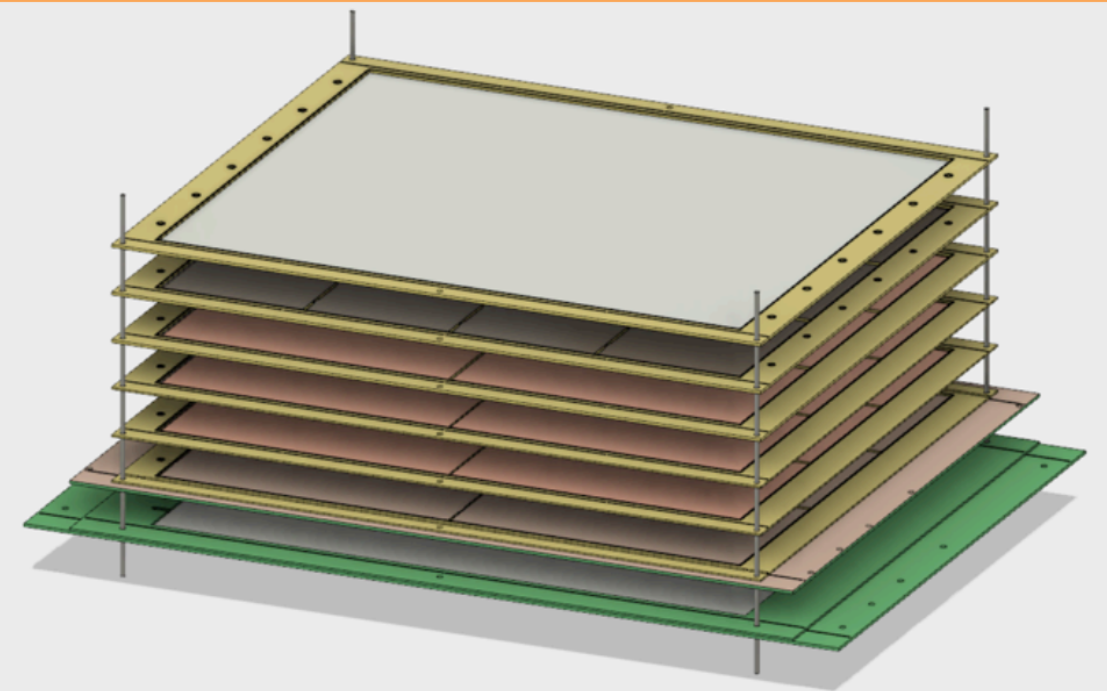
\includegraphics[width=\textwidth]{images/chap5/gem_structure_3d.png}
    \caption{GEM Chamber 2D structure}
  \end{minipage}
  \hfill
  \begin{minipage}[b]{0.45\textwidth}
    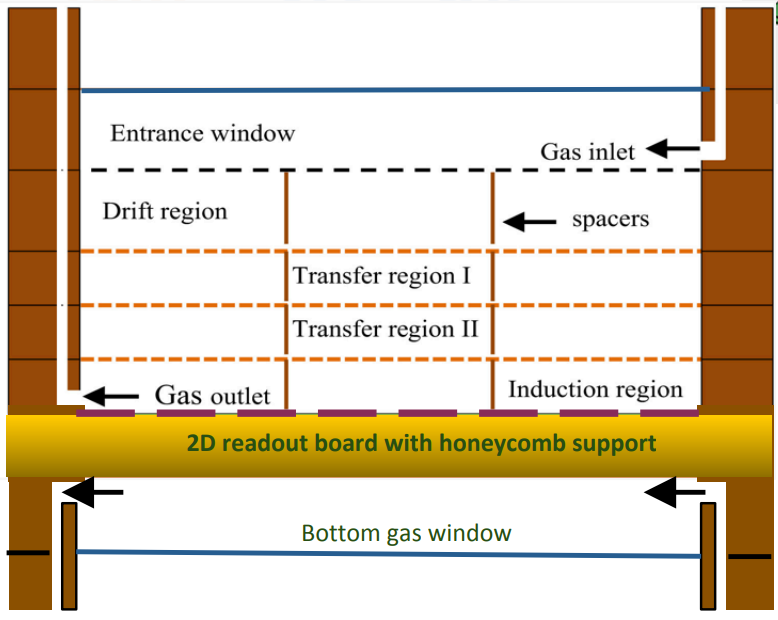
\includegraphics[width=\textwidth]{images/chap5/gem_structure_chamber_2d.png}
    \caption{GEM chamber Gas flow}
  \end{minipage}
\end{figure}


\subsection{GEM Detectors in Hall A High-Resolution Spectrometer}

For PRex/CRex experiments, Each HRS was  equipped with three large SBS GEM detectors, each measuring $50 cm \times 60 cm$, and three smaller GEM detectors measuring $10 cm \times 20 cm$ produced by Idaho State University. As shown  in  Fig.N, the GEM detectors were arranged parallel to each other and placed downstream of  the VDCs, first the Idaho GEM detectors and then  the larger SBS GEM detectors. The primary integrating detectors used for production data collection, two quartz detectors,  were placed between the first and second Idaho GEM detectors, while two AT detectors were situated between the SBS GEM detectors and the Idaho GEM detectors. {\bf NL indicate what type are AT detectors}


\begin{figure}[!htbp]
  \centering
  \begin{minipage}[b]{0.45\textwidth}
    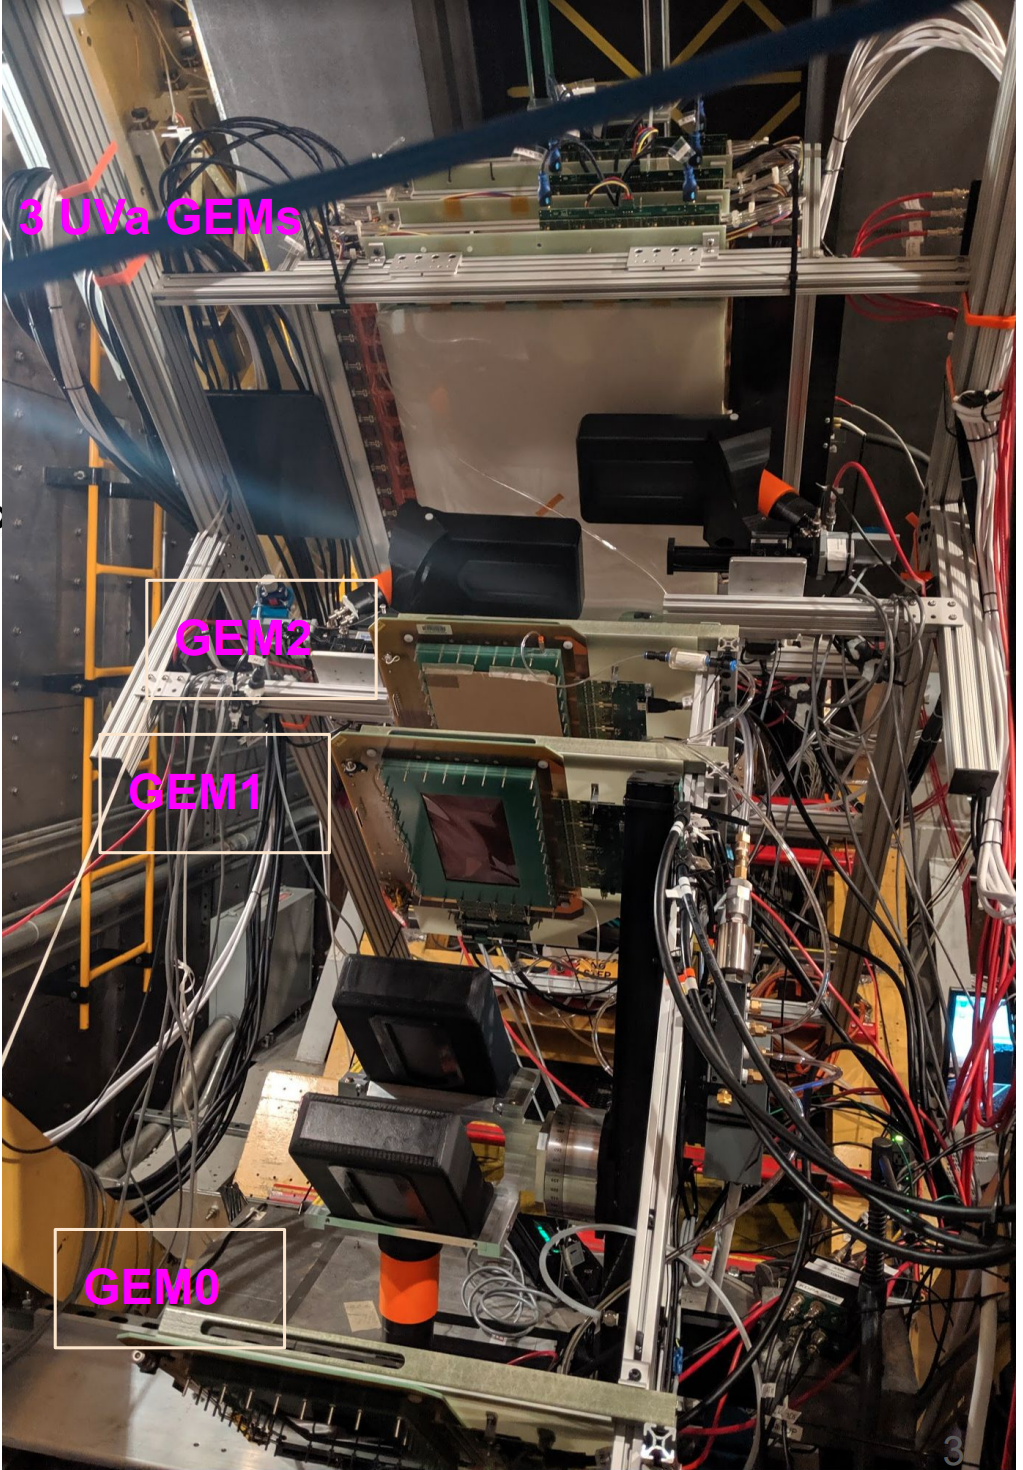
\includegraphics[width=\textwidth]{images/chap5/gem_in_apparatus_photo.png}
    \caption{GEM Chamber 2D structure}
  \end{minipage}
  \hfill
  \begin{minipage}[b]{0.45\textwidth}
    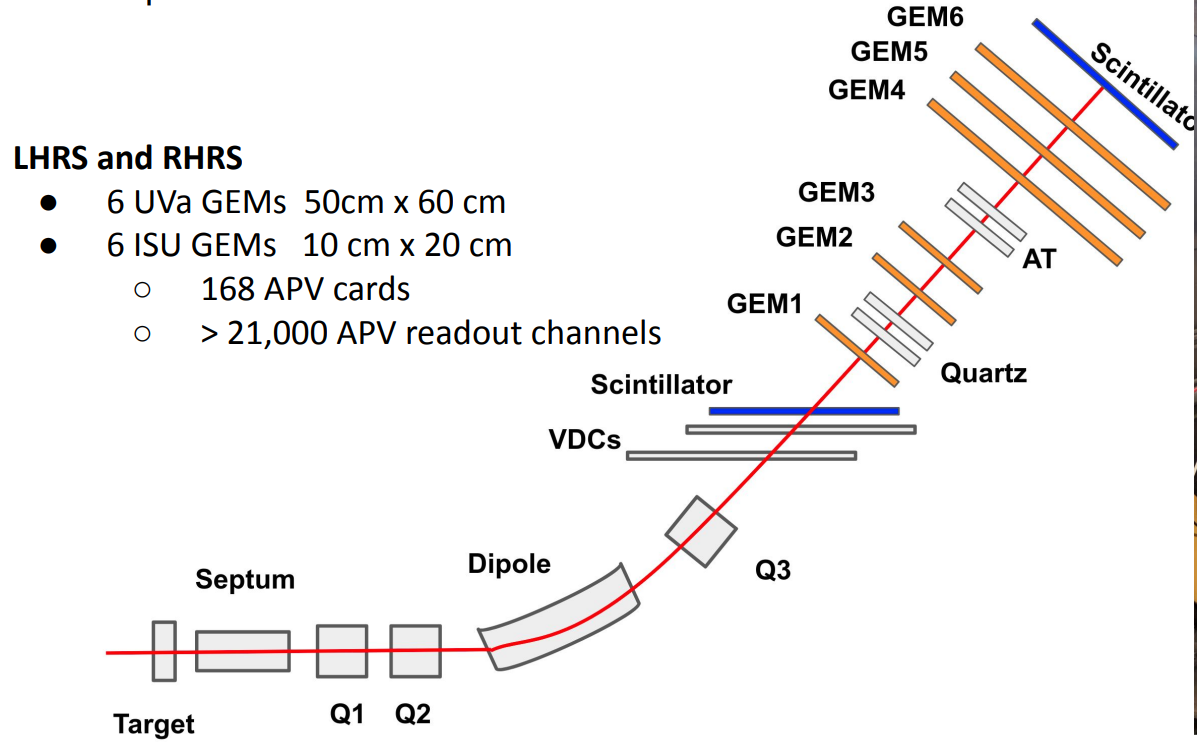
\includegraphics[width=\textwidth]{images/chap5/gem_apparatus_in_hrs_2d.png}
    \caption{GEM chamber Gas flow}
  \end{minipage}
\end{figure}


\subsection{Add a more detailed introduction of GEM detector supplement electronics?? [MOVE TO CHAPTER 3]}
\begin{enumerate}
    \item readout electronics (APV, MPD, CPU, coda)
    \item low voltage for the APV (modular LV, cable selection, LV regulator, cooling fan) 
    \item High Voltage
    \item Gas System
\end{enumerate}


\begin{figure}[!htbp]
  \centering
  \begin{minipage}[b]{0.45\textwidth}
    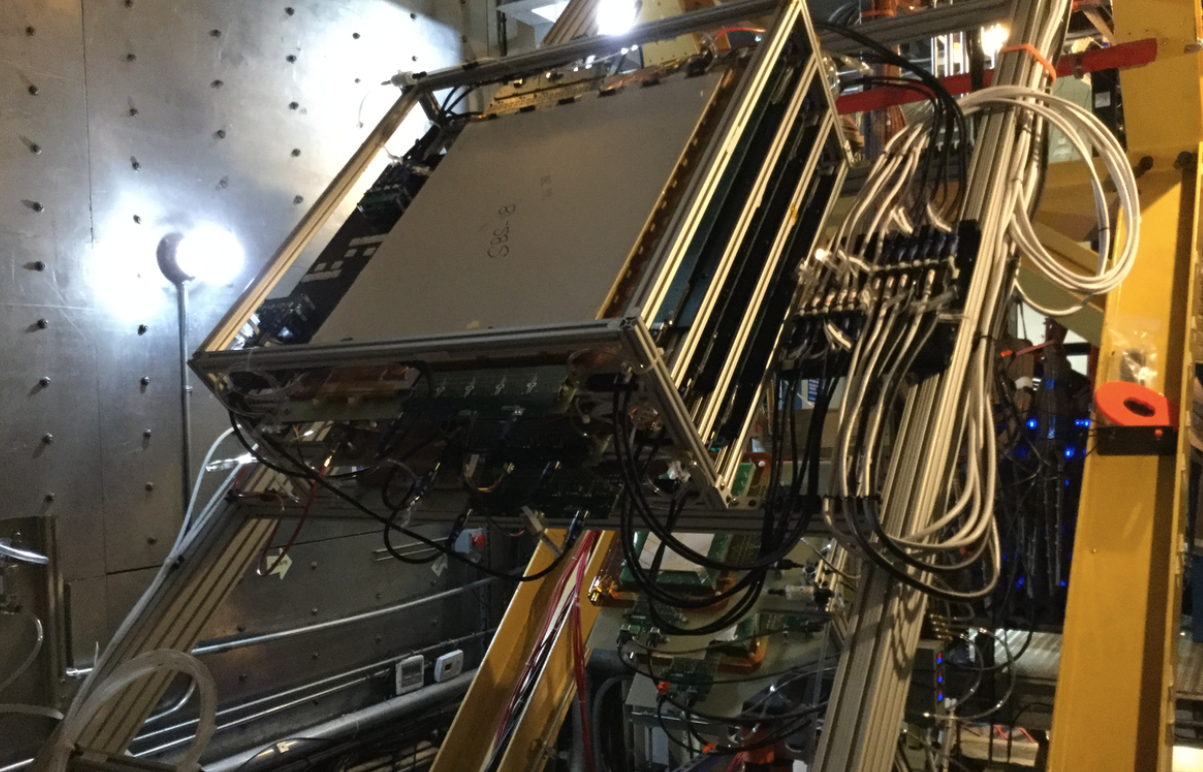
\includegraphics[width=\textwidth]{images/chap5/gem_in_hrs.png}
    \caption{GEM Chamber in HRS}
  \end{minipage}
  \hfill
  \begin{minipage}[b]{0.45\textwidth}
    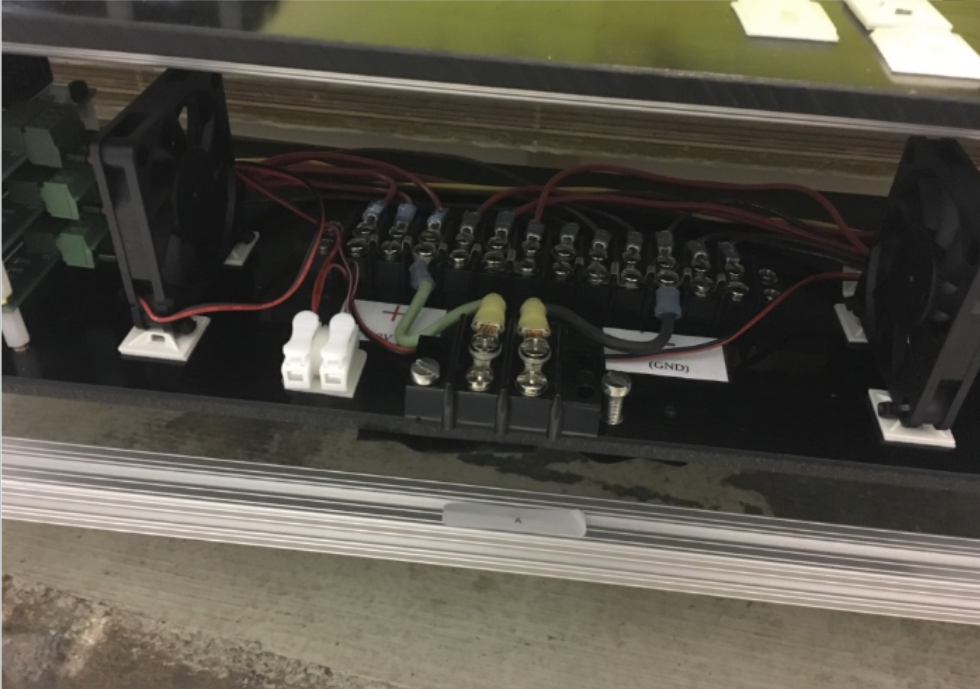
\includegraphics[width=\textwidth]{images/chap5/gem_low_voltage.png}
    \caption{GEM Pre-Amplifier Voltage Supply}
  \end{minipage}
\end{figure}


\begin{figure}
    \centering
    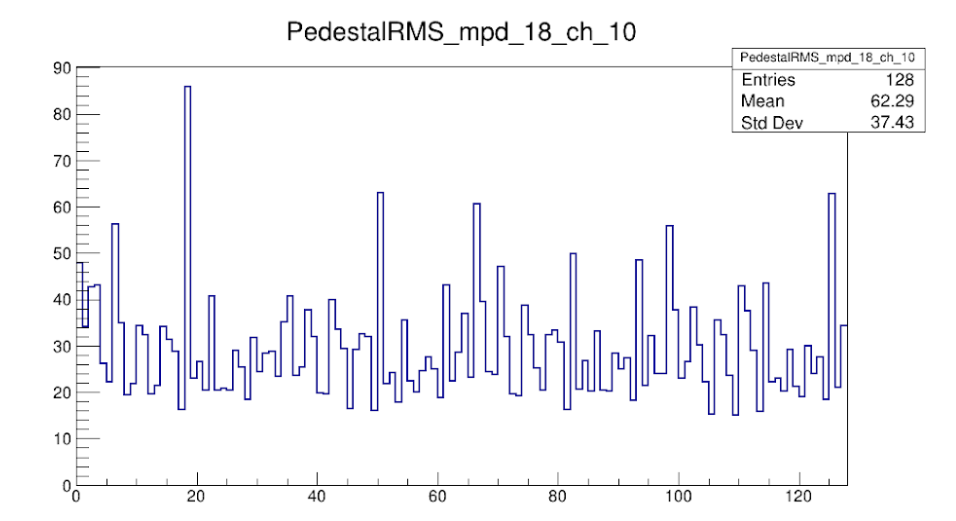
\includegraphics[width=\textwidth]{images/chap5/gem_signal.png}
    \caption{Caption}
    \label{fig:apv_25_pedestal_plot}
\end{figure}

\section{GEM Detector Data Analysis}

The GEM detector readout strips were connected to the APV frontend card. The APV-25 chips is  a 128-channel analog amplifier and multiplexor card. The anaplified analog signals from the 128 channels in the APV chip are multiplexed and time sequenced to a single serial line. This signal train is   transmitted,  via a HDMI cable,  to a Multi-Purpose Digitizer, where it is de-multiplexed and converted to digital signals using a 12-bit Analog to Digital Converter. Figure \ref{fig:apv_25_pedestal_plot} displays a typical plot after MPD conversion. {\bf NL: for this you need to show  a real signal plot, not pedestal} The x-axis represents the APV channels, and the y-axis corresponds to the ADC values after the conversion, which are proportional to the amount  of charge collected by the given strip.

To extract useful signals from these raw signals, multiple steps have to be  employed, including common mode subtraction, pedestal measurement, and fired strip selection using zero suppression.

\subsection{GEM Pedestal Measurement}

A pedestal run involves setting the high voltage to 2000 V for a dry run. At this high voltage, the electric field is insufficient to trigger an avalanche, meaning no signals should be detected on the readout strips. By applying a 2000 V high voltage ensures that  the noise from the high voltage modules  are included  when estimating the pedestal, as opposed to having no high voltage applied. The pedestal of each channel of the 128 APV channels is calculated by subtracting the ADC value from the common mode, defined as the average of the 128-channel ADC values. Subsequently, the Root Mean Square (RMS) and mean of each channel's pedestal are computed across all the events that have been recorded.

Figure \ref{fig:lhrs_pedestal_distribution} and \ref{fig:rhrs_pedestal_distribution} shows the pedestal distributions of all  channels used in the PRex experiment. The x-axis represents the index of the APV card, and the y-axis corresponds to the RMS value of the pedestal. Each data point in the plot represents one GEM readout channel.

The first 18 APV cards are utilized in the Idaho GEM detectors. As the area of these detectors is $10 cm \times 20 cm$, their pedestal RMS values are also smaller than those of the SBS GEM detectors. The LHRS GEM detectors have larger pedestal RMS values than those of the RHRS, with RMS values of around 20 ADC, which equates to approximately $0.02 V$ voltage fluctuation. A few channels in each APV card exhibit much higher pedestals, and these are considered dead channels due to issues in the Printed Circuit Board (PCB) manufacturing process.

\begin{figure}[!htbp]
    \centering
    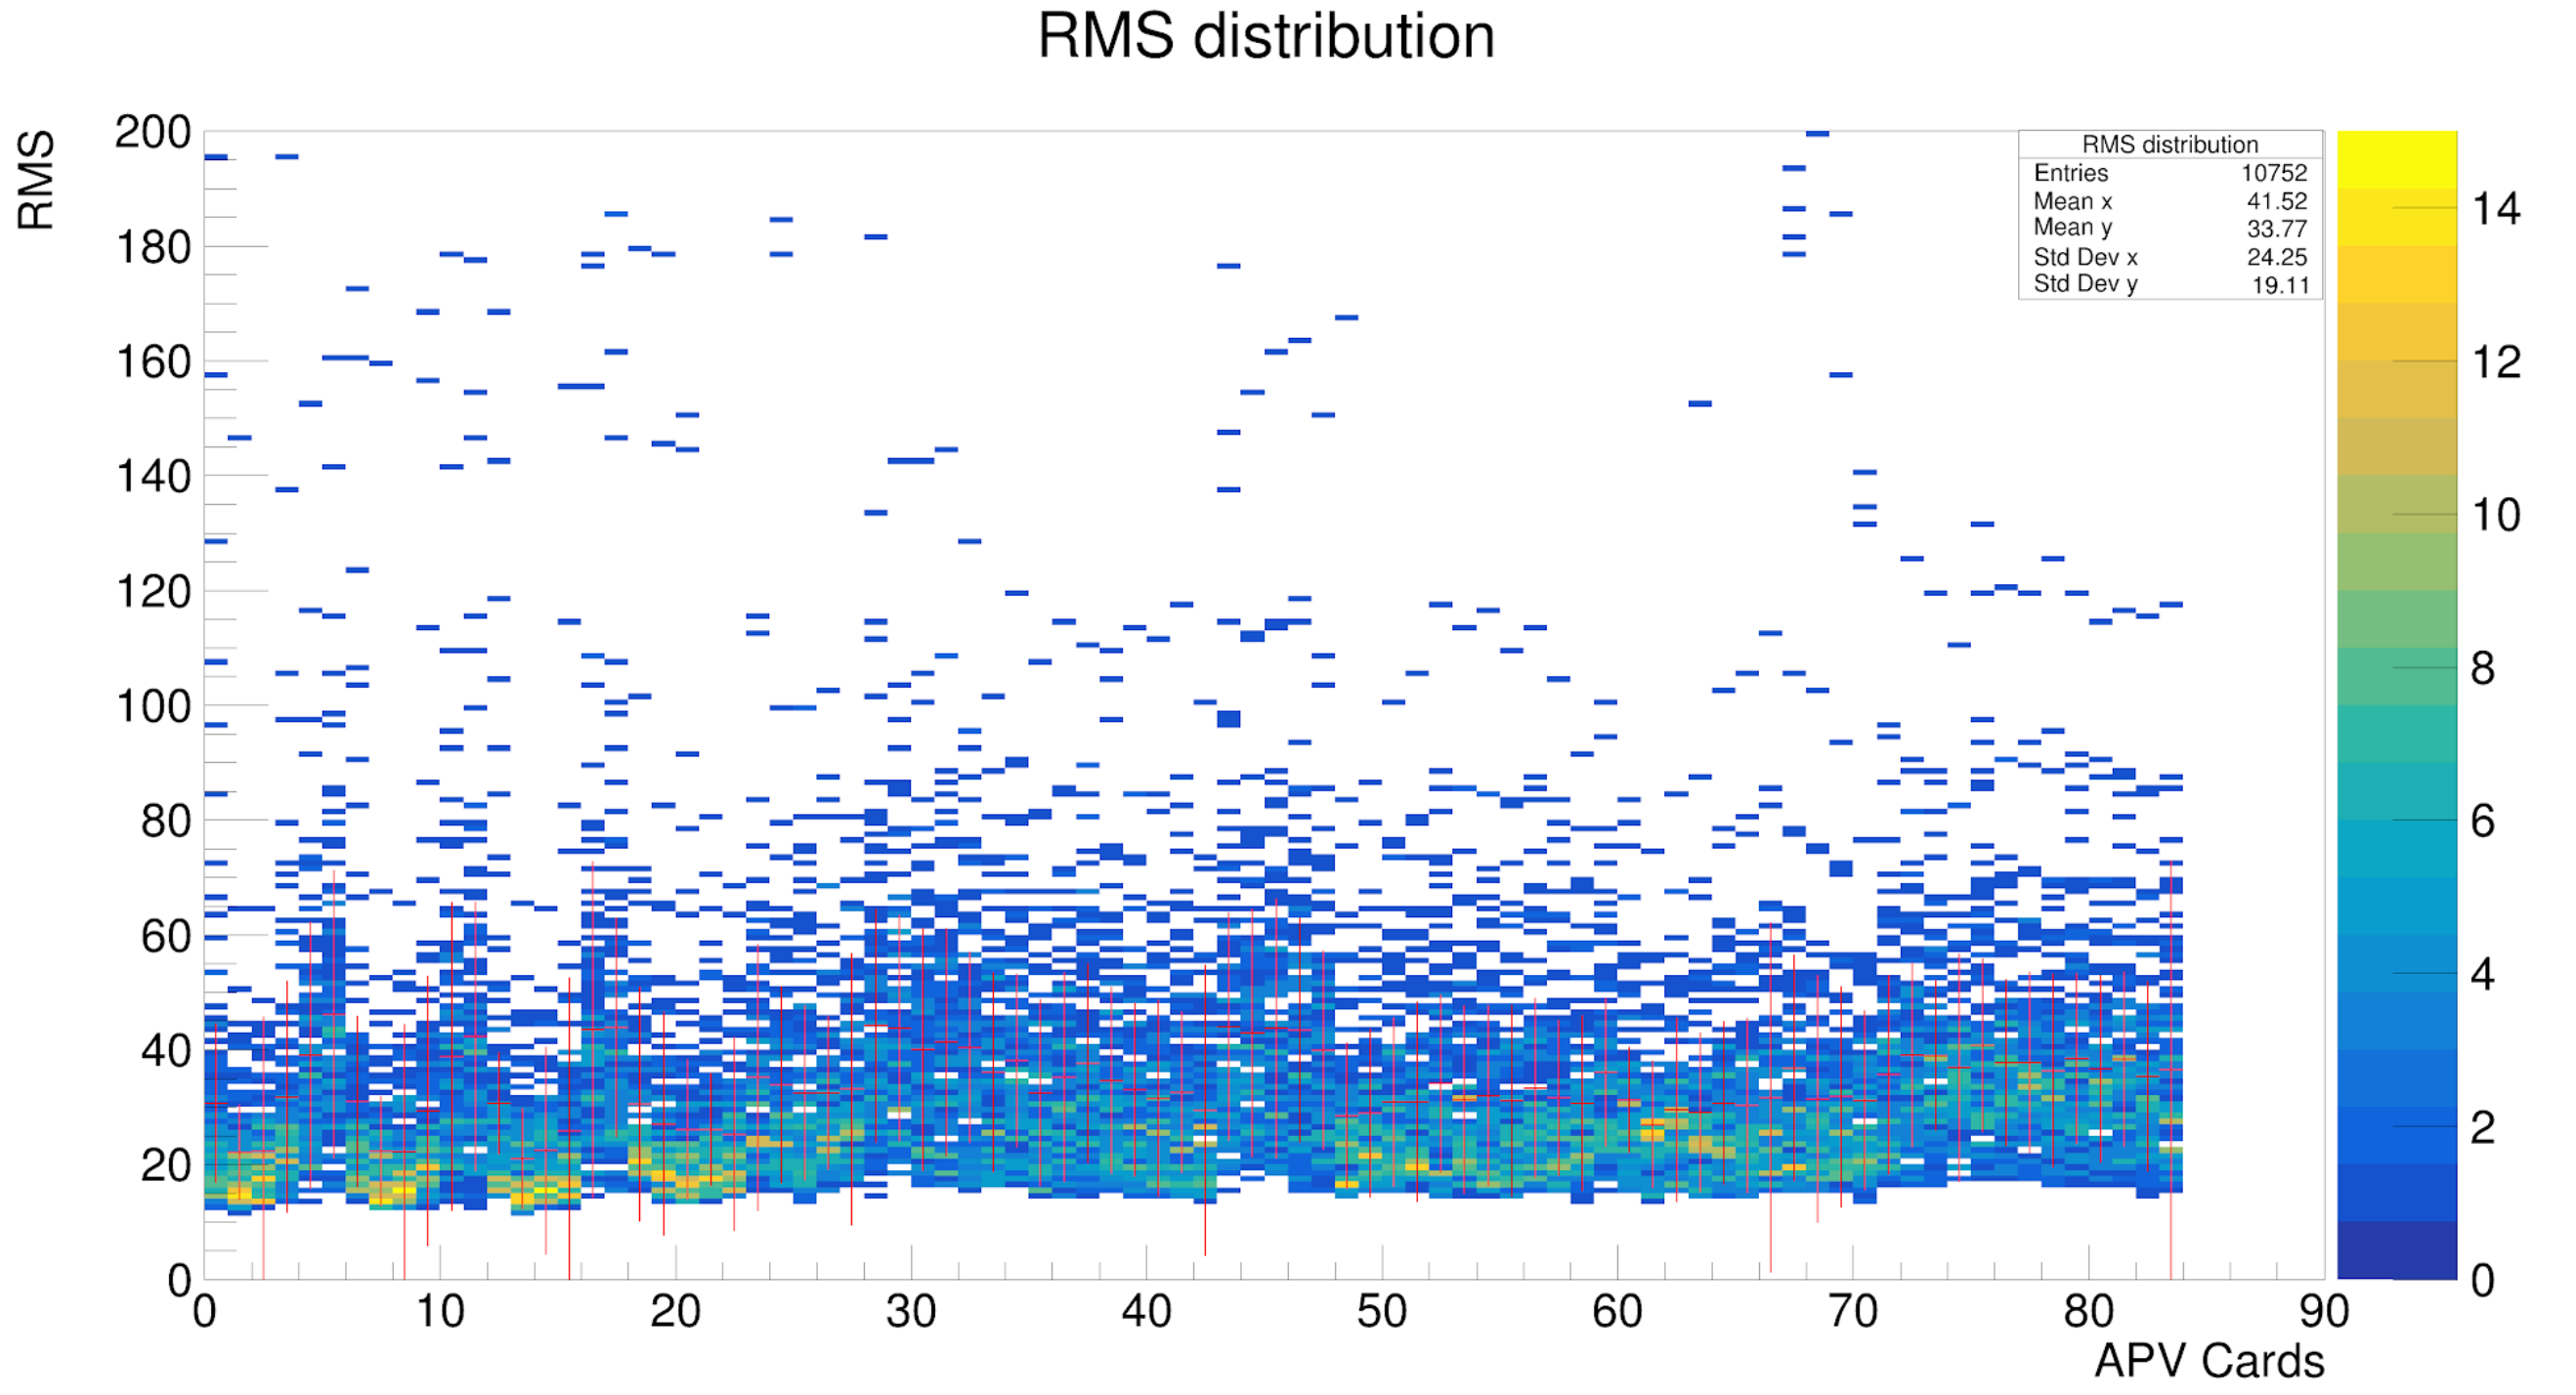
\includegraphics[width=\textwidth]{images/chap5/LHRS_pedestal.png}
    \caption{LHRS GEM Readout RMS of Pedestal Distribution}
    \label{fig:lhrs_pedestal_distribution}
\end{figure}

\begin{figure}[!htbp]
    \centering
    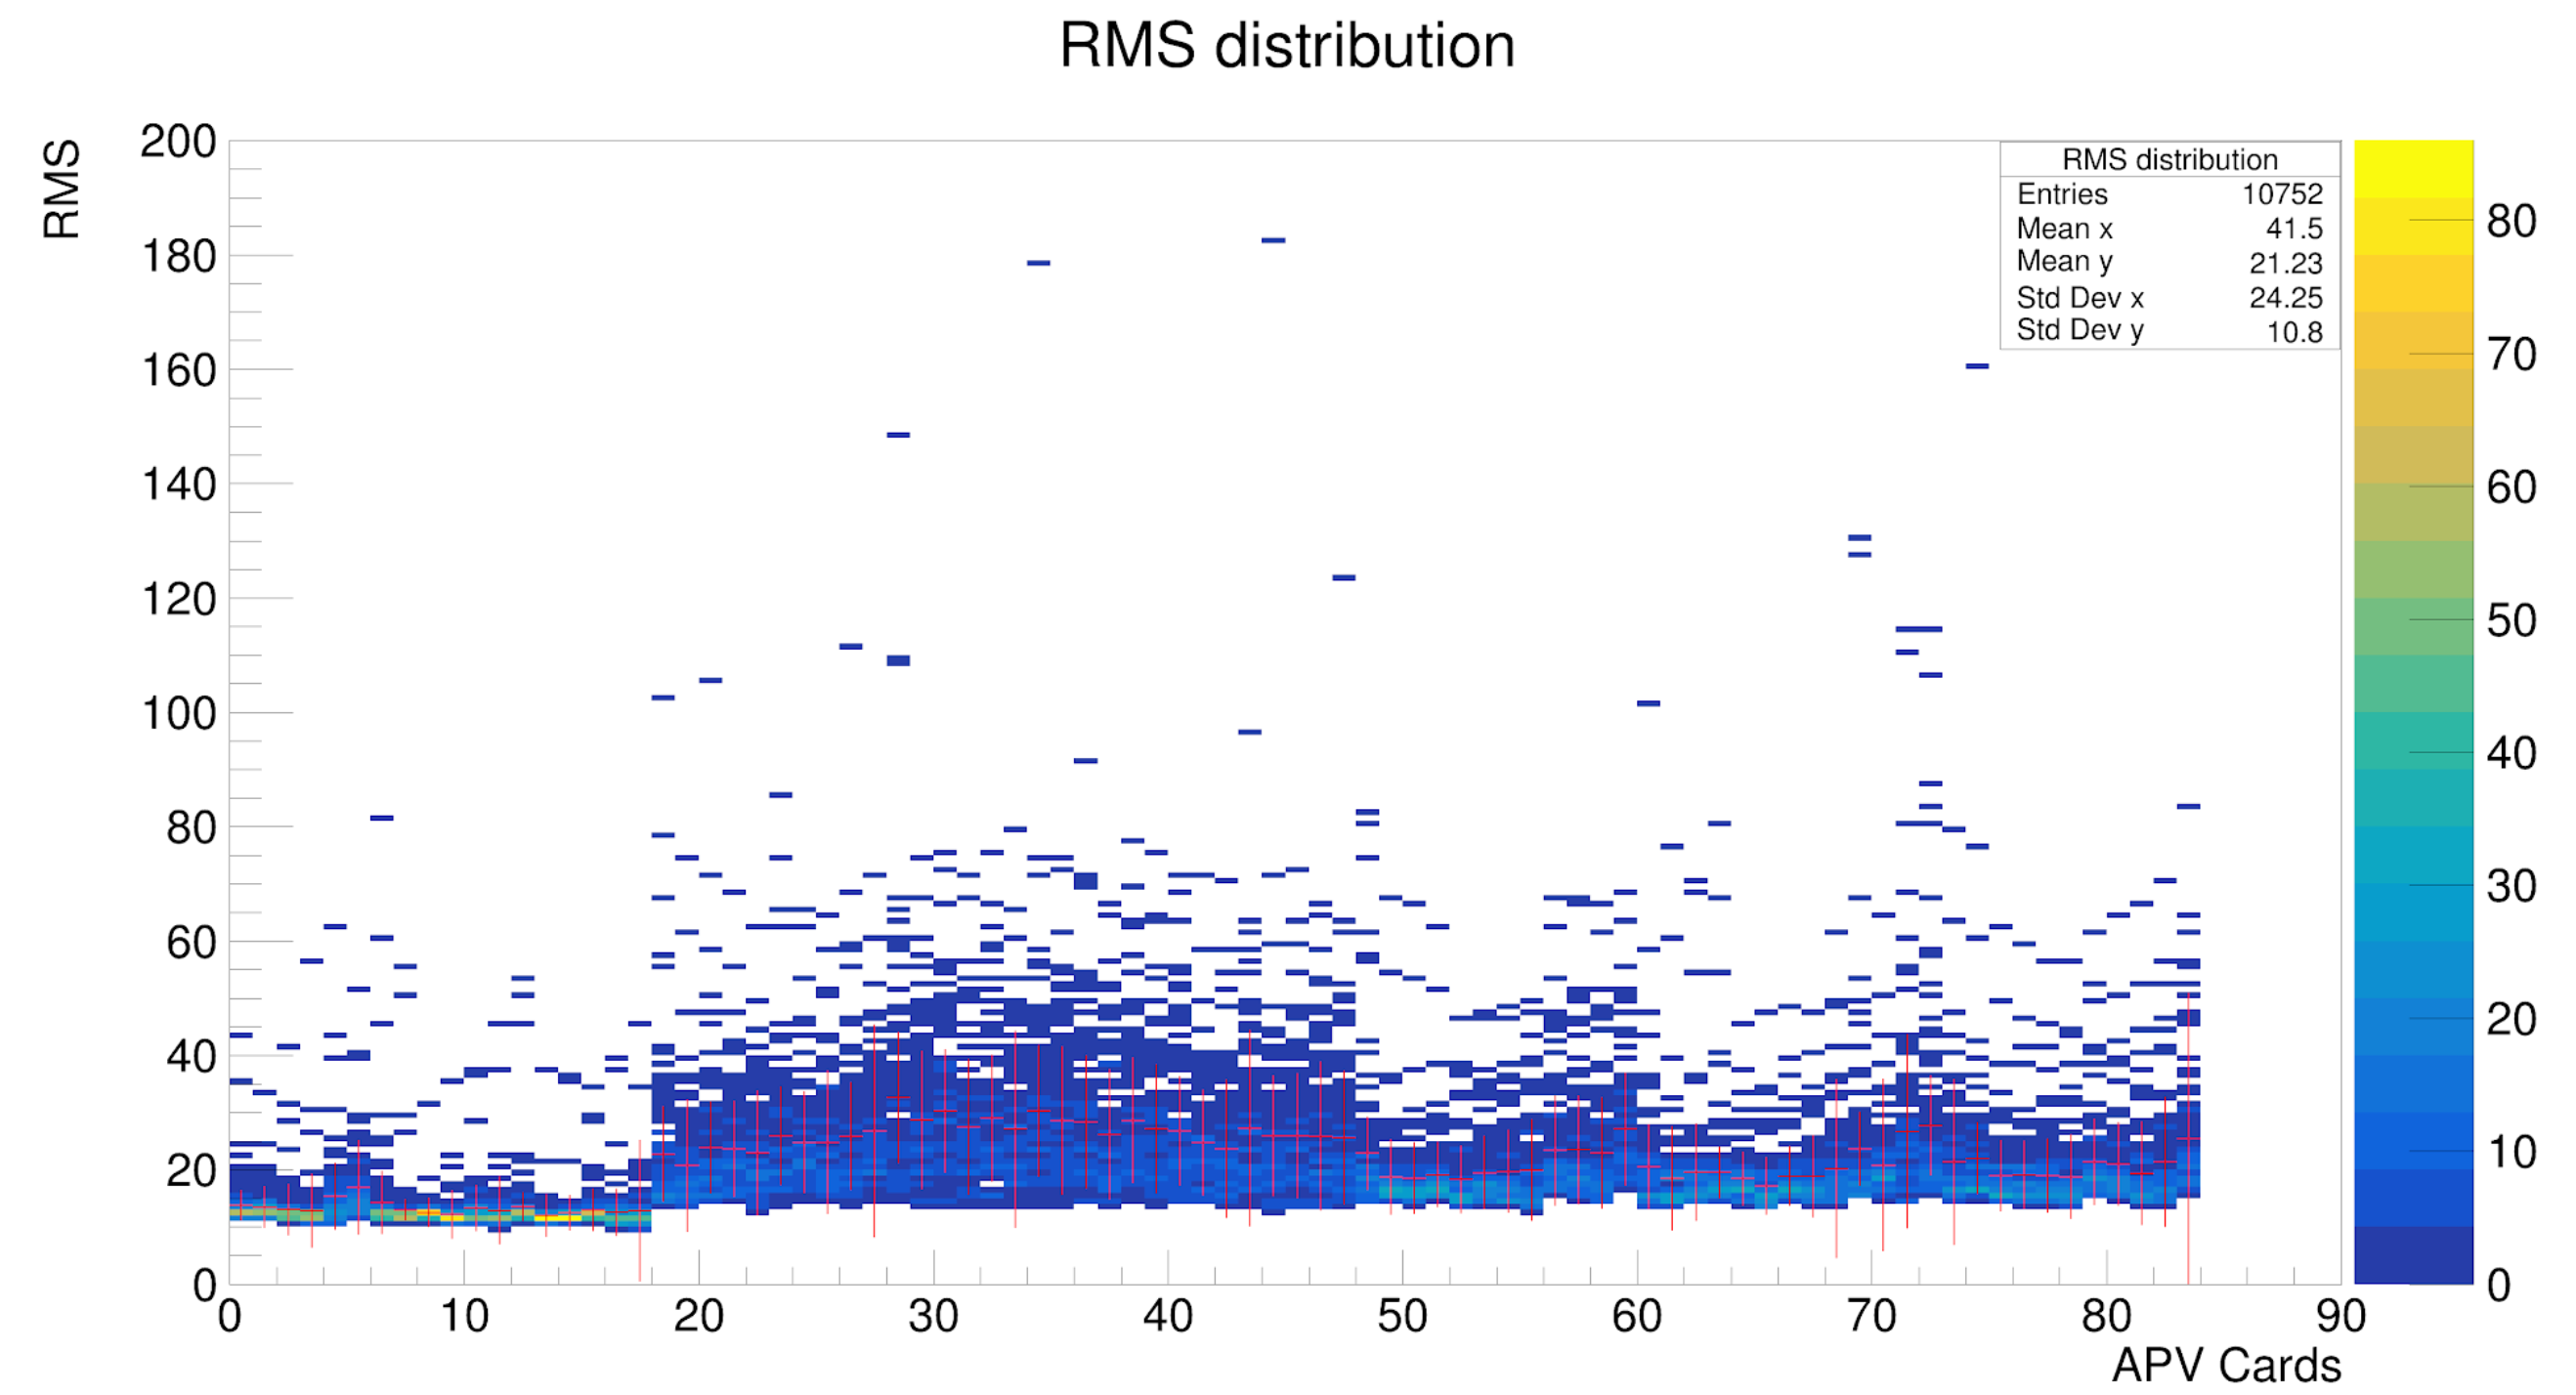
\includegraphics[width=\textwidth]{images/chap5/rhrs_pedestal.png}
    \caption{RHRS GEM Readout RMS of Pedestal Distribution}
    \label{fig:rhrs_pedestal_distribution}
\end{figure}

{\bf NL: Siyu:  I edited the following section while offline flying on the plane; please replace your material with that I have here }


\subsection{GEM Pedestal Measurement}

A pedestal run involves setting the high voltage to 2000 V for a dry run. At this high voltage, the electric field is insufficient to trigger an avalanche, meaning no signal should be detected on the readout strips. By applying a 2000 V high voltage, the noise from the high voltage modules can be considered when estimating the pedestal, as opposed to having no high voltage applied. The pedestal of each channel of the 128 APV channels is calculated by subtracting the ADC value from the common mode, defined as the average of the 128-channel ADC values. Subsequently, the Root Mean Square (RMS) and mean of each channel's pedestal are computed across all  events that have been recorded.

Figure \ref{fig:lhrs_pedestal_distribution} and \ref{fig:rhrs_pedestal_distribution} show the pedestal distributions of all the channels used in the PRex experiment. The x-axis represents the index of the APV card, and the y-axis corresponds to the RMS value of the pedestal. Each data point in the plot represents one GEM readout channel.

The first 18 APV cards are utilized in the Idaho GEM detectors. As the area of these detectors is $10 cm \times 20 cm$, their pedestal RMS values are also smaller than those of the SBS GEM detectors. The LHRS GEM detectors have larger pedestal RMS values than those of the RHRS, with RMS values of around 20 ADC, which equates to approximately $0.02 V$ voltage fluctuation. A few channels in each APV card exhibit much higher pedestals, and these are considered dead channels due to issues in the Printed Circuit Board (PCB) manufacturing process.

\begin{figure}[!htbp]
    \centering
    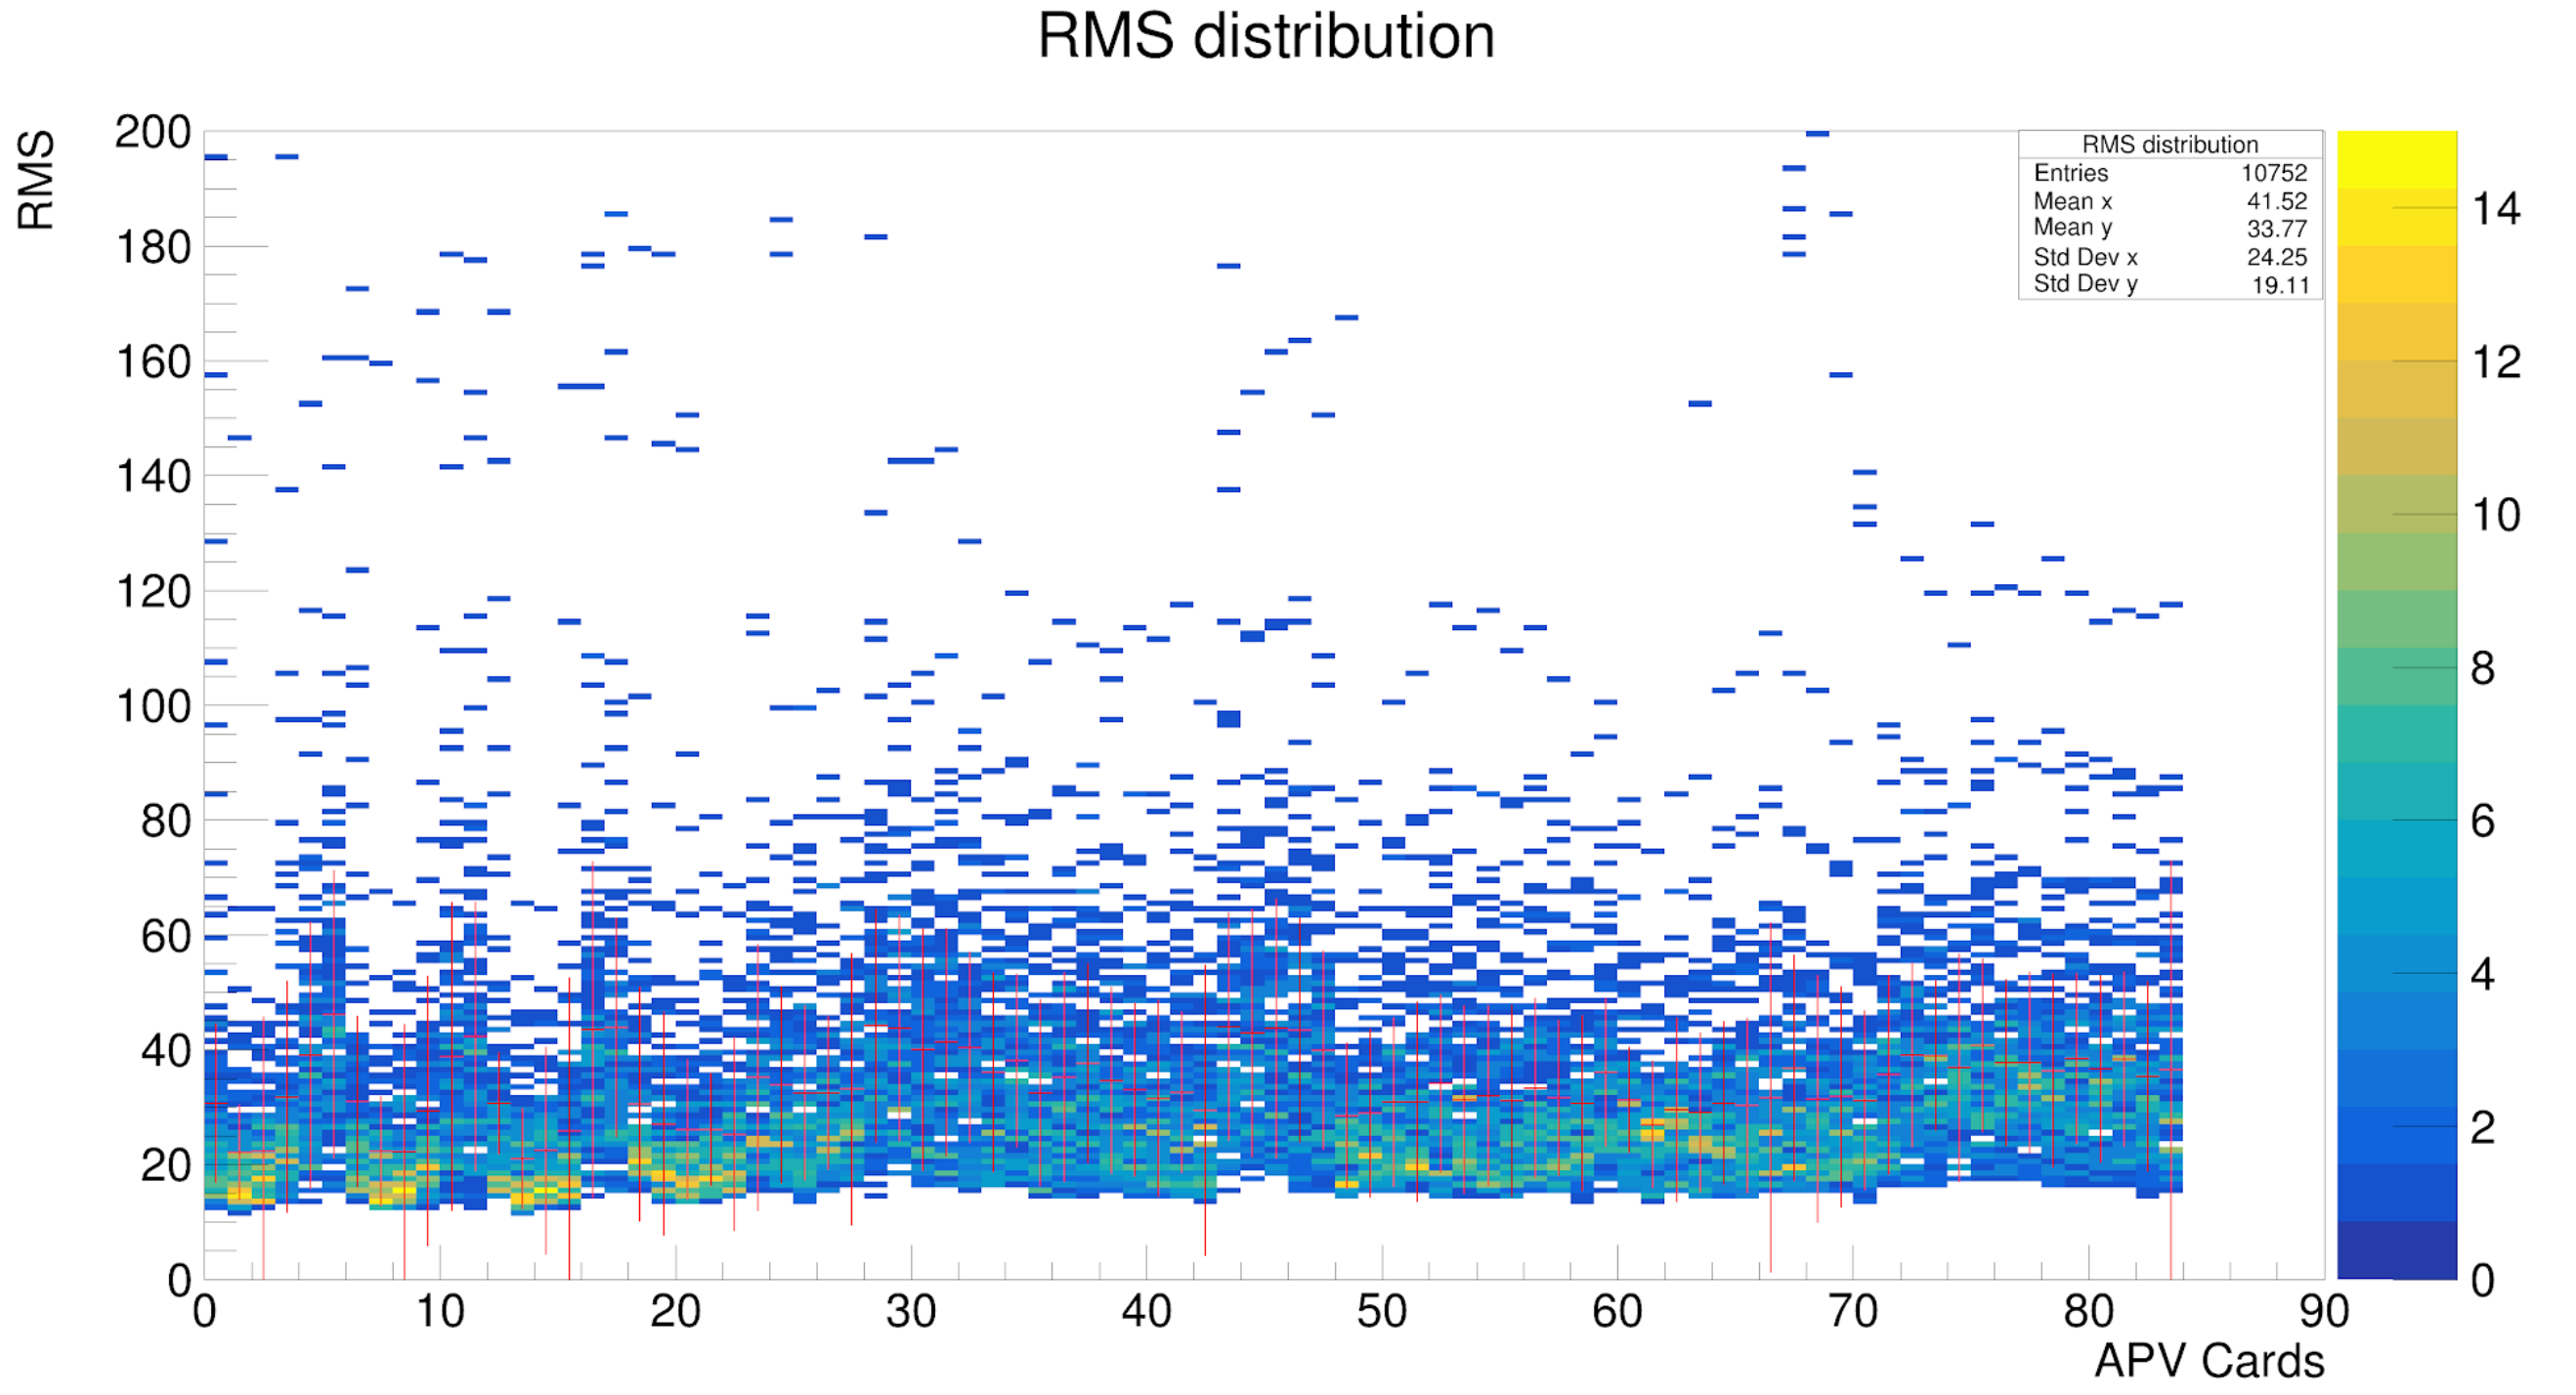
\includegraphics[width=\textwidth]{images/chap5/LHRS_pedestal.png}
    \caption{LHRS GEM Readout RMS of Pedestal Distribution}
    \label{fig:lhrs_pedestal_distribution}
\end{figure}

\begin{figure}[!htbp]
    \centering
    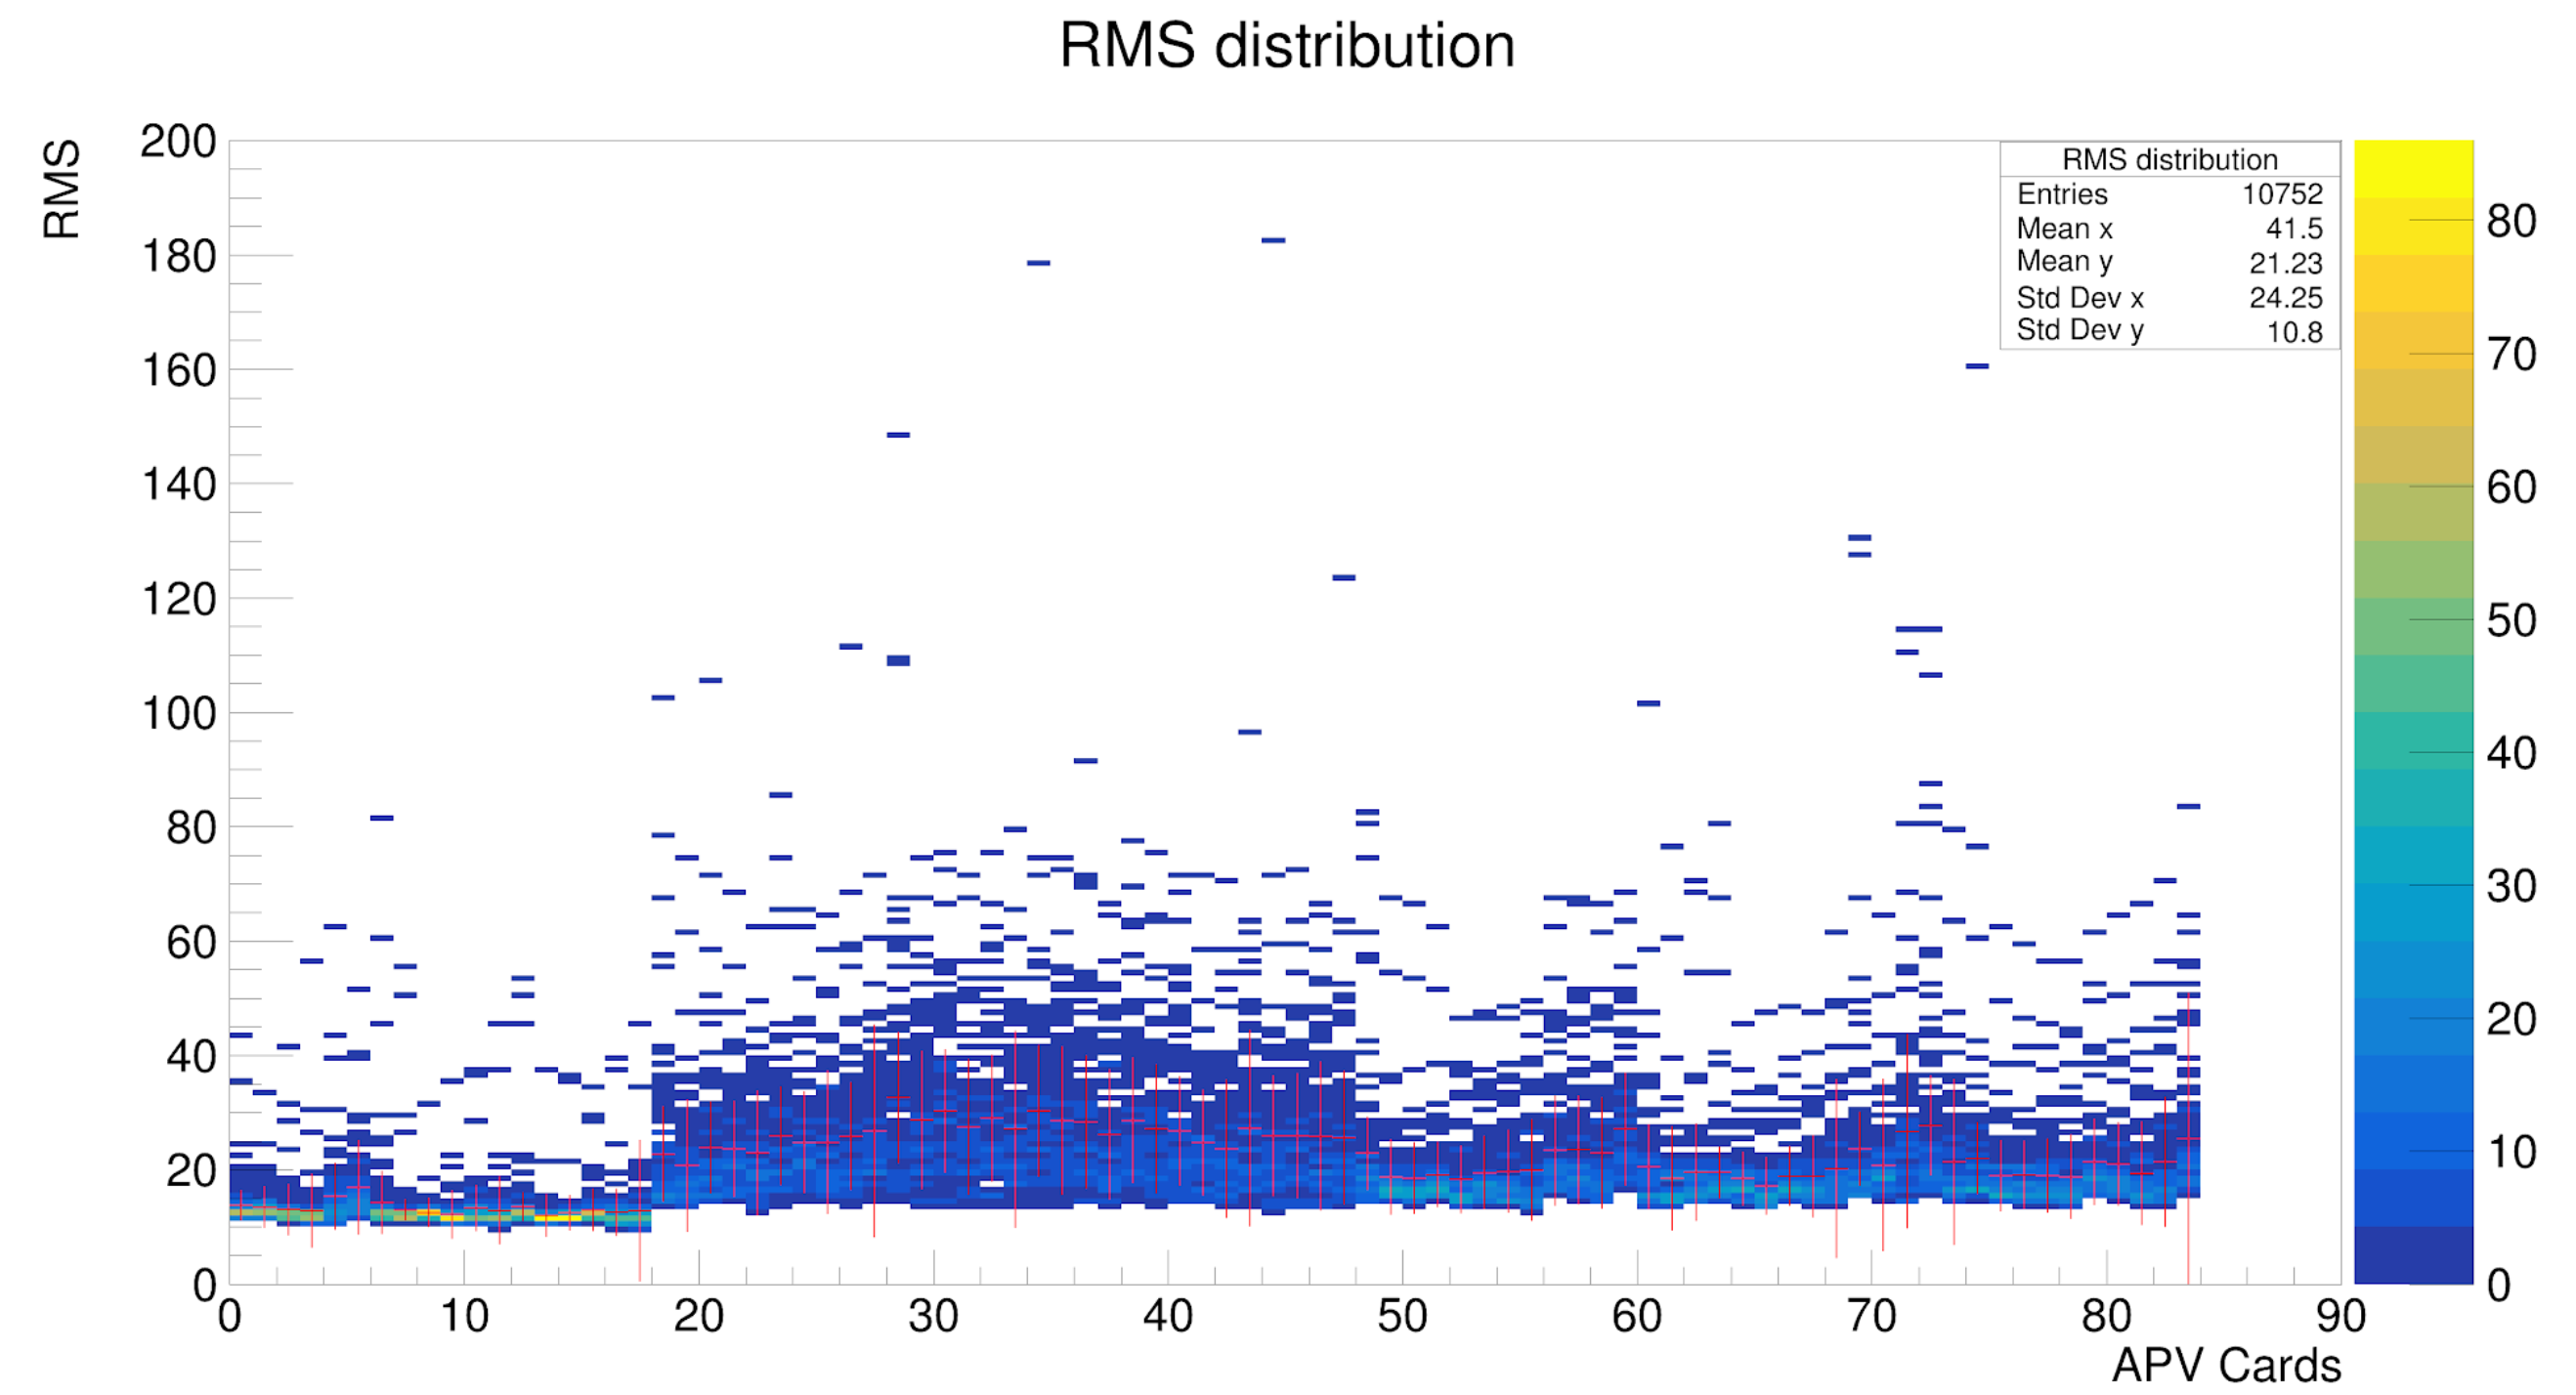
\includegraphics[width=\textwidth]{images/chap5/rhrs_pedestal.png}
    \caption{RHRS GEM Readout RMS of Pedestal Distribution}
    \label{fig:rhrs_pedestal_distribution}
\end{figure}


\subsubsection{GEM detector false positive rate}

When the GEM detector works at Normal working voltage. When a particle passes through  
the GEM detectors and ionized the gases inside the GEM chambers. The ionized electrons 
will travel along the Electric field and get amplified within the holes in GEM detectors, 
and then the avalanche electrons will be collected by the readout strips and readout with the electronics. 

The common mode correction of raw signal ADC values is done using the same algorightm as
 in the case of pedestal ADCs. After that, the pedestal corrected ADC value for each strip is
calculated by  subtracting  the mean of the pedestal for that strip from the common mode 
corrected ADC value. The determination of fired  GEM  strips is achieved  
by comparing the corrected ADC  values with the pedestal thresholds. Different channels may have different 
noise performances, for example,  due to different strip capacitances.  To get a consistent criterion,
 the threshold for a  given channel is chosen to be N $\times$ (RMS of the pedestal).  
If the value is larger than the threshold, then the  given strip is  considered to have fired,
 and the strip number along with  its corrected ADC value are written into the fired strip array.  
If the corrected ADC value is lower than the threshold, then the correctd ADC value for that strip 
is set to zero, and the strip is marked as non-fired. The constant N was typically set to 5 for 
SBS GEM modules used in PRex/CRex exeperiments. 

Setting the threshold   too high with a high value of N increases the probability of  actually  fired 
good signal  strips to  be categorized as  non-signal  (False Negative), leading to artificial reduction 
of detection efficiency.  On the other hand, if the threshold is set too low, it increases the the 
 chance that pedestal  noise is categorized as good signals from fired strips (False Positive). 

To measure the false positive rate, the GEM signal selection algorithm was applied on a 2000 V voltage 
dry run, other than the dry run used for the pedestal calculation. Since there are no real signals  at 
2000 V,  any fired strips in this run are false positive signals. By measuring the ratio of the fired 
strips in the dry run total number of triggers, we can estimate the False Positive Rate of the algorithm. 
In fig \ref{fig:lhrs_fake_hit_rate} and \ref{fig:rhrs_fake_hit_rate} are the false positive  hit rate 
for the SBS GEM detectors on LHRS and RHRS. At the $5\sigma$ threshold, the false hit rate for LHRS 
was $0.16\%$ and $0.01\%$.

{\bf NL: end of offline edited section}

\subsubsection{GEM detector false positive rate}

When the GEM detector works at Normal working voltage. When a particle passes through  the GEM detectors and ionized the gases inside the GEM chambers. The ionized electrons will travel along the Electric field and get amplified within the holes in GEM detectors, and then the avalanche electrons will be collected by the readout strips and readout with the electronics. 

Similar to the algorithm used for calculating the pedestals, the signals will first subtract the common mode. After that, the value of the strips is calculated by subtracting the value from the corresponding mean of the pedestals. The determination of GEM fired strip is determined by comparing the calculated values with the threshold. Different channels may have different noise performances, to get a consistent criterion, the threshold of given channels is chosen to be n*rms of the pedestal. If the value is larger than the threshold, the given strips are considered to be fired strips. 

If the threshold is too high, there is more chance fired strip to categorized to be non-signal (False Negative), on the other hand, if the threshold is set too low, the is more chance a white noise will be categorized to be fired strips (False Positive). 

To measure the false positive rate, the GEM signal selection algorithm is applied on a 2000v voltage dry run. At 2000v there should no real signals, if there is any triggered strips, those are fake fired signals. By measuring the ratio of the fired strips in the dry run, we can estimate the False Positive Rate of the algorithm. In fig \ref{fig:lhrs_fake_hit_rate} and \ref{fig:rhrs_fake_hit_rate} are the fake hit rate for the SBS GEM detectors on the LHRS and Right HRS. At the $5\sigma$ threshold, the fake hit rate for left HRS is $0.16\%$ and $0.01\%$.

\subsubsection{High Voltage Scan Efficiency for GEM detectors}
\subsubsection{GEM detector number of cluster performance}
\subsubsection{GEM detector cluster size performance}


\begin{figure}[!htbp]
    \centering
    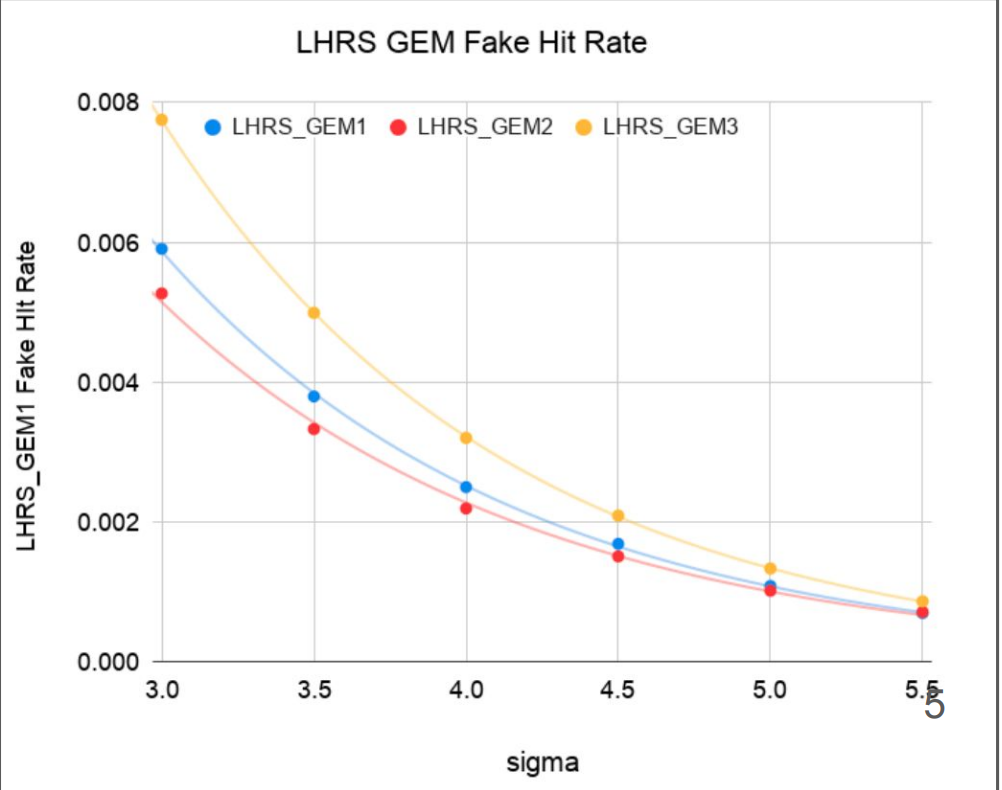
\includegraphics[width=\textwidth]{images/chap5/lhrs_fake_hit_rate.png}
    \caption{LHRS SBS GEM False Hit Rate}
    \label{fig:lhrs_fake_hit_rate}
\end{figure}

\begin{figure}[!htbp]
    \centering
    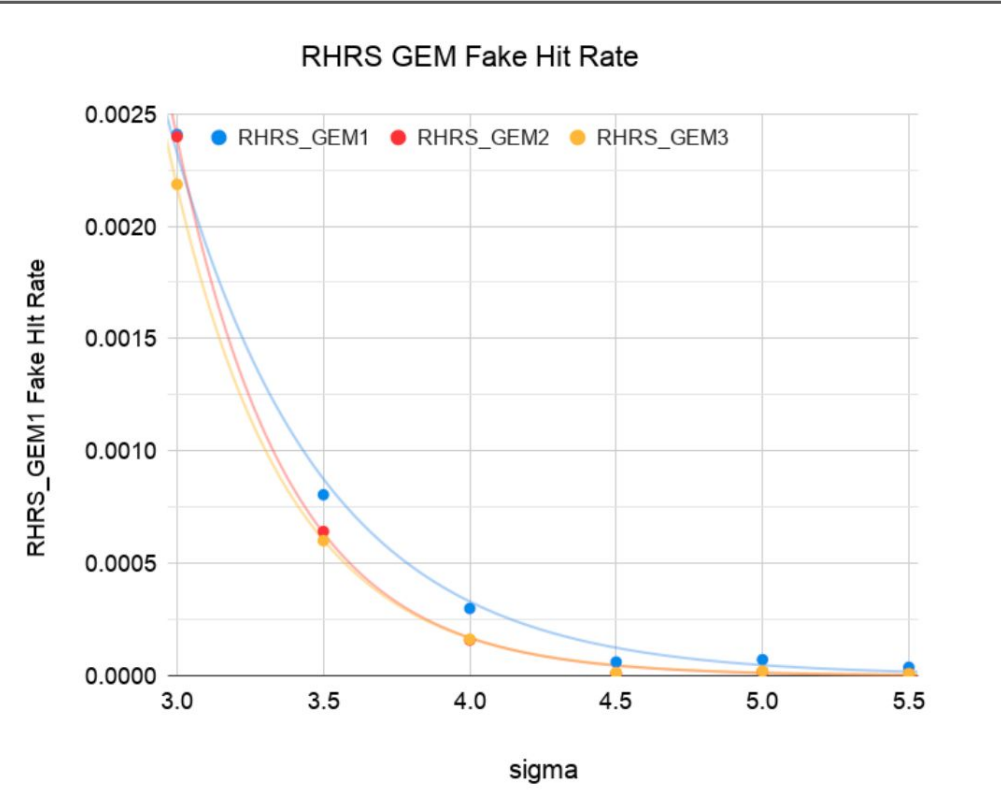
\includegraphics[width=\textwidth]{images/chap5/rhrs_fake_hit_rate.png}
    \caption{RHRS SBS GEM False Hit Rate}
    \label{fig:rhrs_fake_hit_rate}
\end{figure}

\subsection{GEM detector alignment}

\subsubsection{tree search algorithm used for search for the GEM cluster}
\subsubsection{Multiple GEM detectors alignment algorithm }
\subsection{GEM detector performance}

The GEM detectors in the spectrometer serve as an excellent supplement to the VDC detectors employed for tracking scattered electrons. An accurate measurement of the position dependant efficiency profile of the tracking detectors is crucial for evaluating the average Q$2$ for the Pb or Ca elastic peak.  Both the VDC and GEM detectors can provide scattered electron tracks, enabling us to use the reconstructed VDC tracks  to project onto a given GEM detector and measure that  GEM detector's efficiency.

In this section, we will discuss the detailed measurement of GEM efficiency using the tracking method and compare the high-rate performance of the GEM and VDC detectors.

\subsubsection{GEM Detector Efficiency with Tracking}

Each HRS has four layers of VDC chambers, providing highly accurate position and angular information for the track. Taking the VDC as a reference, we project the track reconstructed from the Vertical Drift Chamber onto each GEM detector. We then search for events within a $4 cm \times 4 cm$ area (justify the choice of a 4x4 area instead of a smaller one). If an event is present within the area, it is considered a True Positive event; if not, it is considered a False Negative due to the GEM detector's efficiency. Figures \ref{fig:lhrs_efficiency_2d} and \ref{fig:rhrs_efficiency_2d} display the GEM detector efficiency for LHRS and RHRS, respectively.

\begin{table}[]
    \centering
    \begin{tabular}{c|c|c|c|c|c|c} \hline
         ~ & GEM 1 & GEM 2 & GEM 3 & GEM 1 & GEM 2 & GEM 3 \\ \hline 
         RHRS & $96\%$ & $96\%$ & $96\%$ & $92\%$& $92\%$& $92\%$  \\ \hline
         LHRS & $86\%$& $84\%$ & $87\%$ & $88\%$ & $66\%$ & $92\%$ \\ \hline
    \end{tabular}
    \caption{GEM Detector efficiency}
    \label{tab:gem_detector_efficiency_table}
\end{table}

\begin{figure}[!htbp]
    \centering
    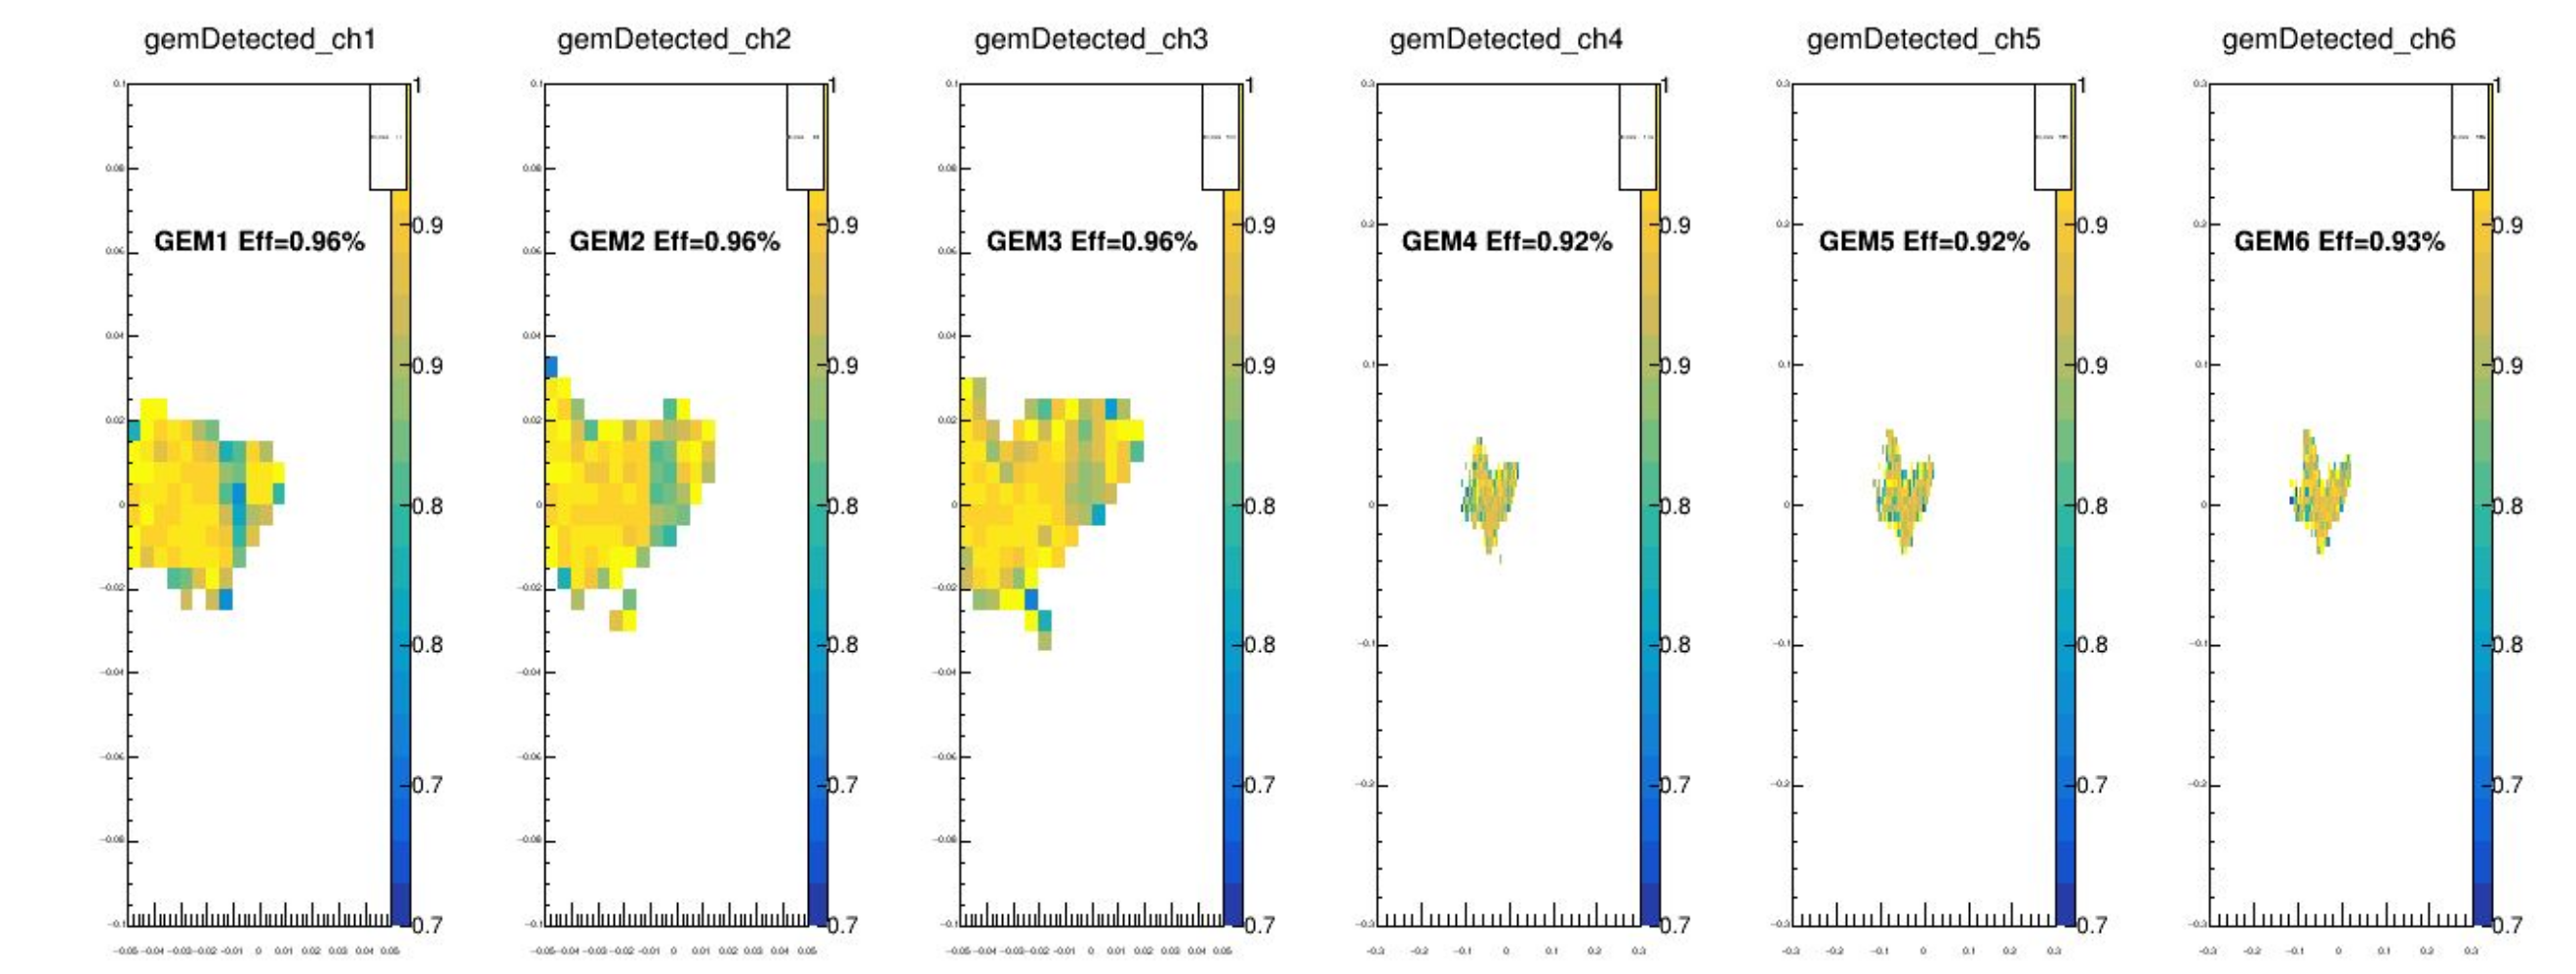
\includegraphics[width=\textwidth]{images/chap5/lhrs_efficiency_2d.png}
    \caption{LHRS GEM detector efficiency}
    \label{fig:lhrs_efficiency_2d}
\end{figure}

\begin{figure}[!htbp]
    \centering
    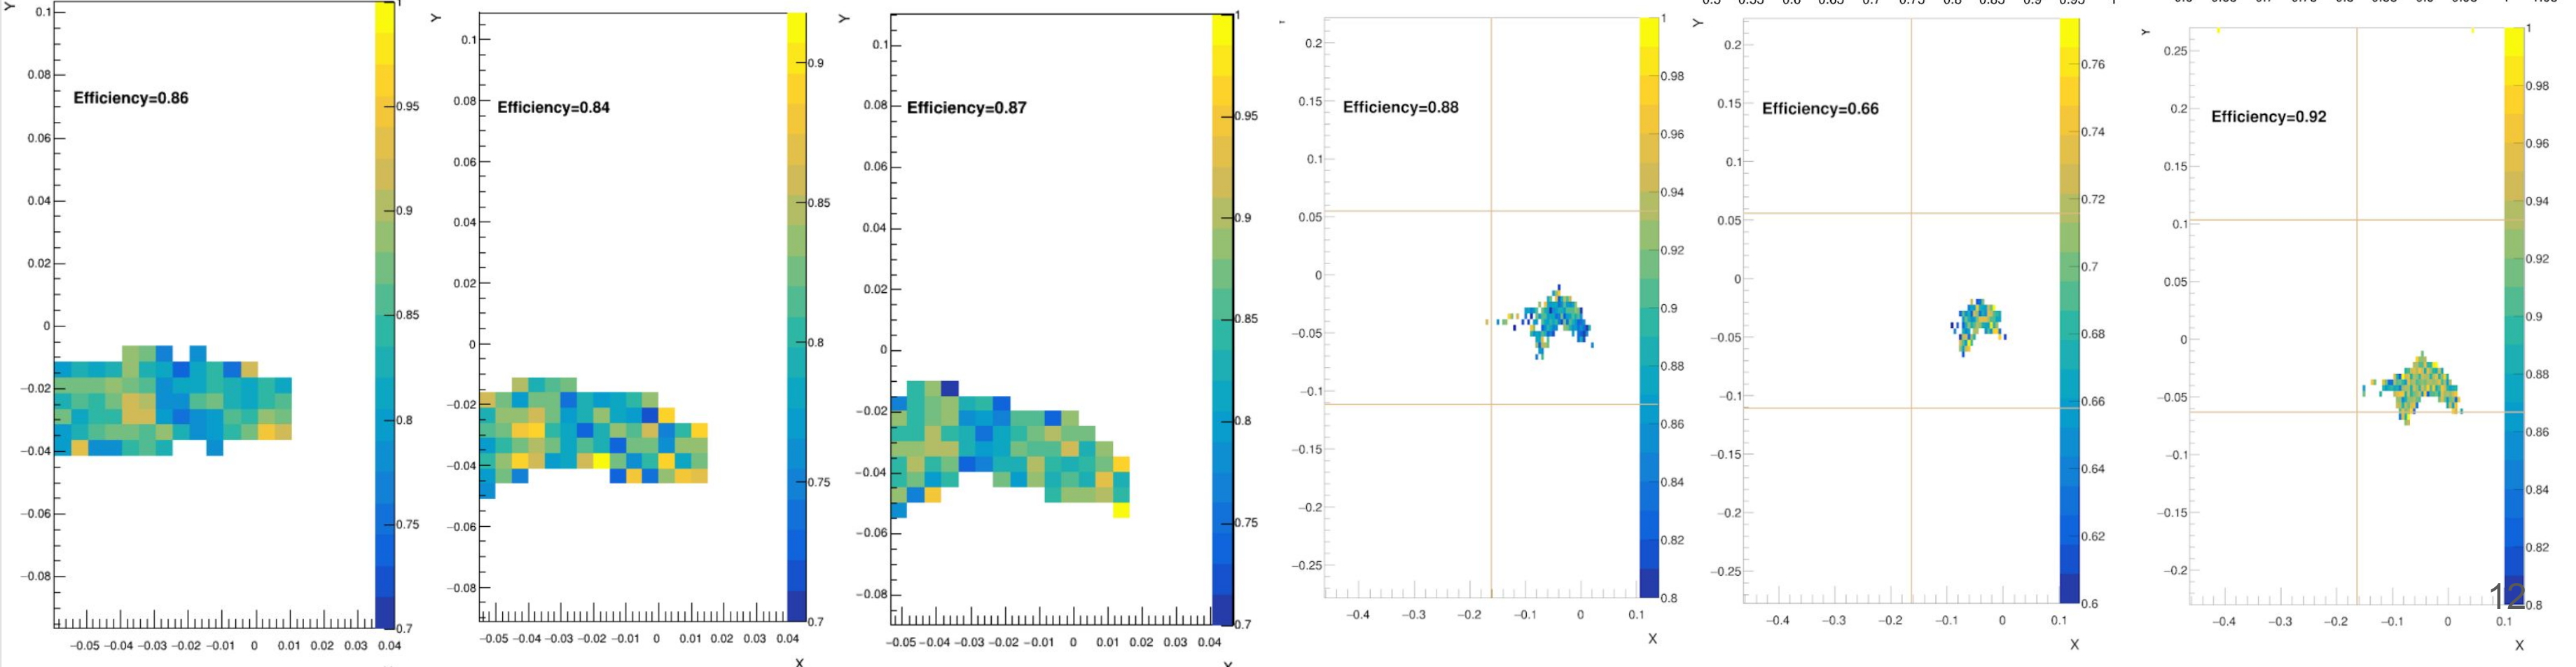
\includegraphics[width=\textwidth]{images/chap5/rhrs_efficiency_2d.png}
    \caption{RHRS GEM detector efficiency}
    \label{fig:rhrs_efficiency_2d}
\end{figure}

To get a better understanding of the efficiency difference by each area, the GEM detector is divided by $1cm \times 1cm$ bin. The efficiency of each bin is computed individually. Figure \ref{fig:lhrs_gem_bin_efficiency} and \ref{fig:rhrs_gem_bin_efficiency} is the efficiency distribution.  
\begin{figure}[!htbp]
    \centering
    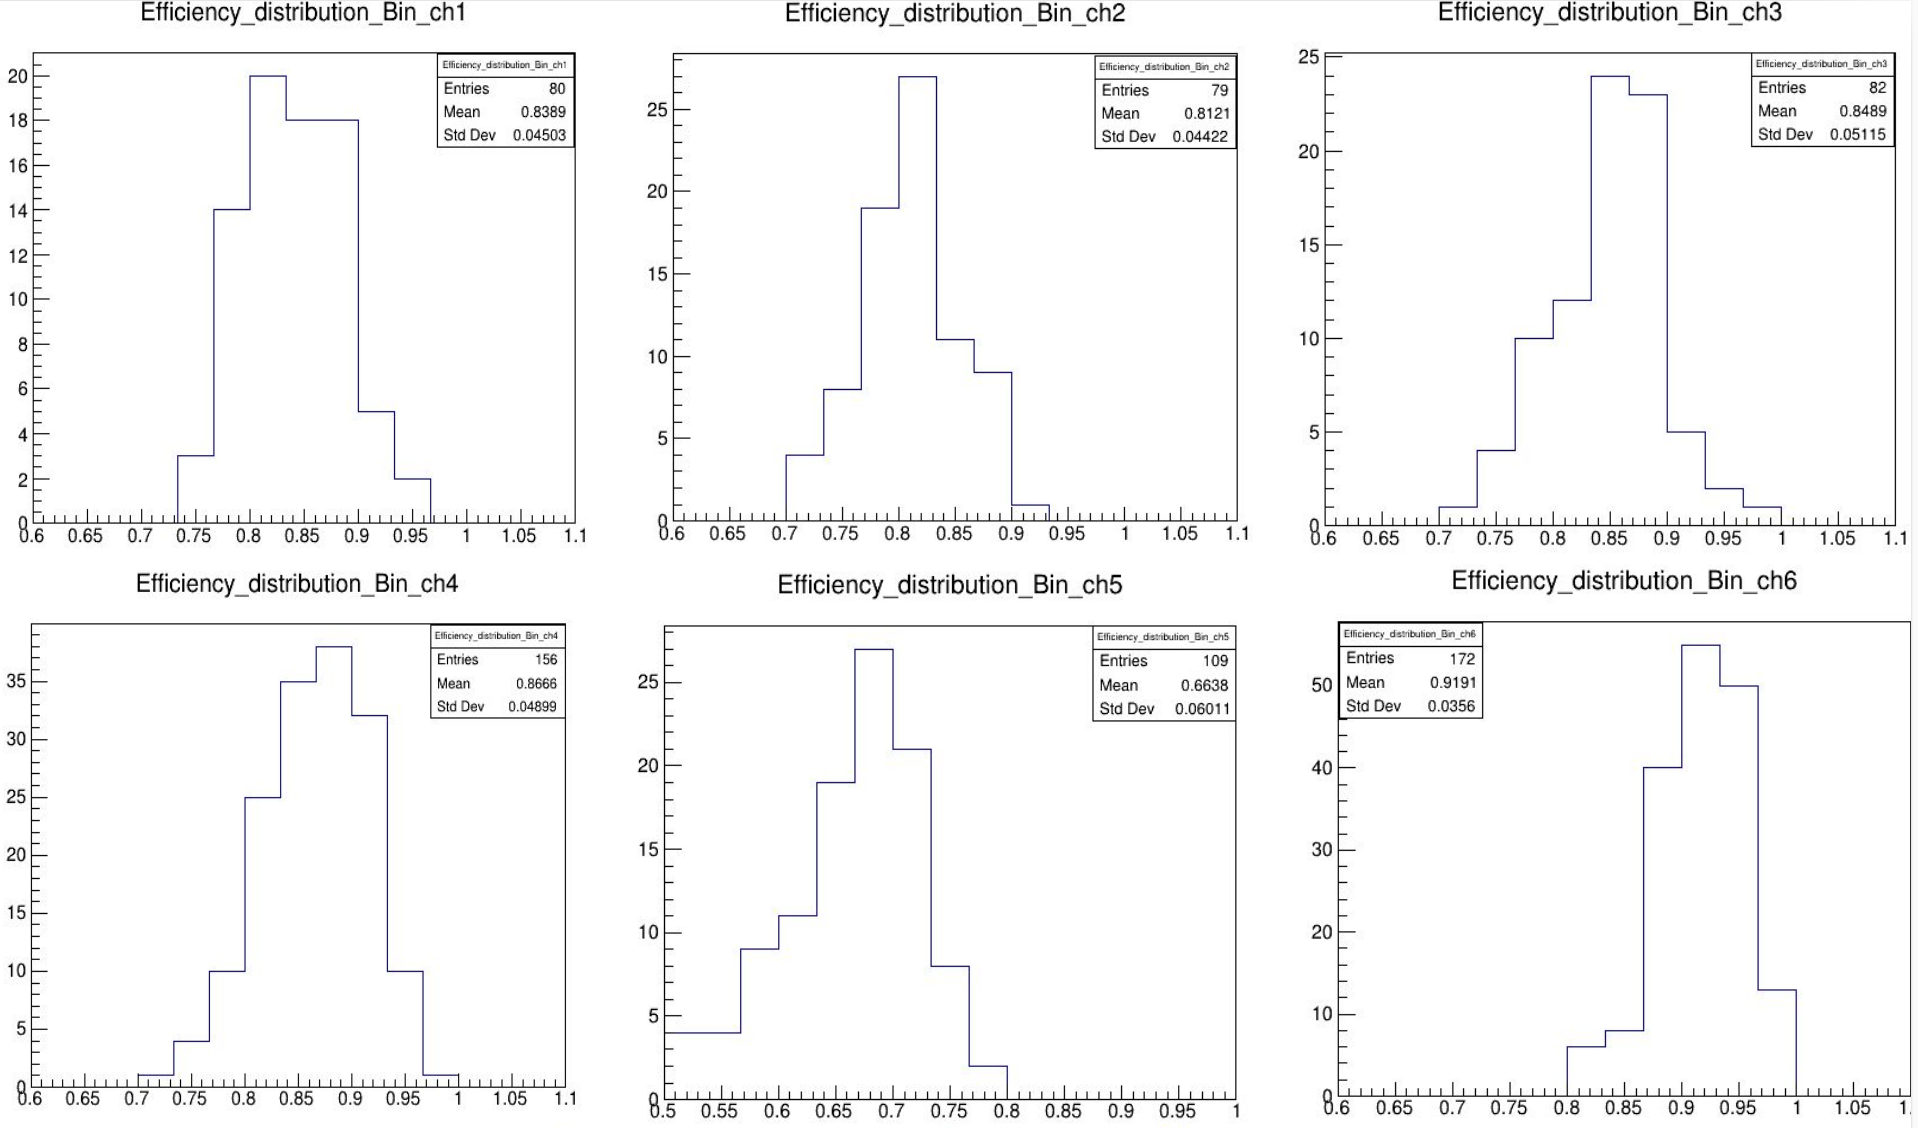
\includegraphics[width=\textwidth]{images/chap5/lhrs_gem_bin_efficiency.png}
    \caption{GEM Efficiency distribution}
    \label{fig:lhrs_gem_bin_efficiency}
\end{figure}

\begin{figure}[!htbp]
    \centering
    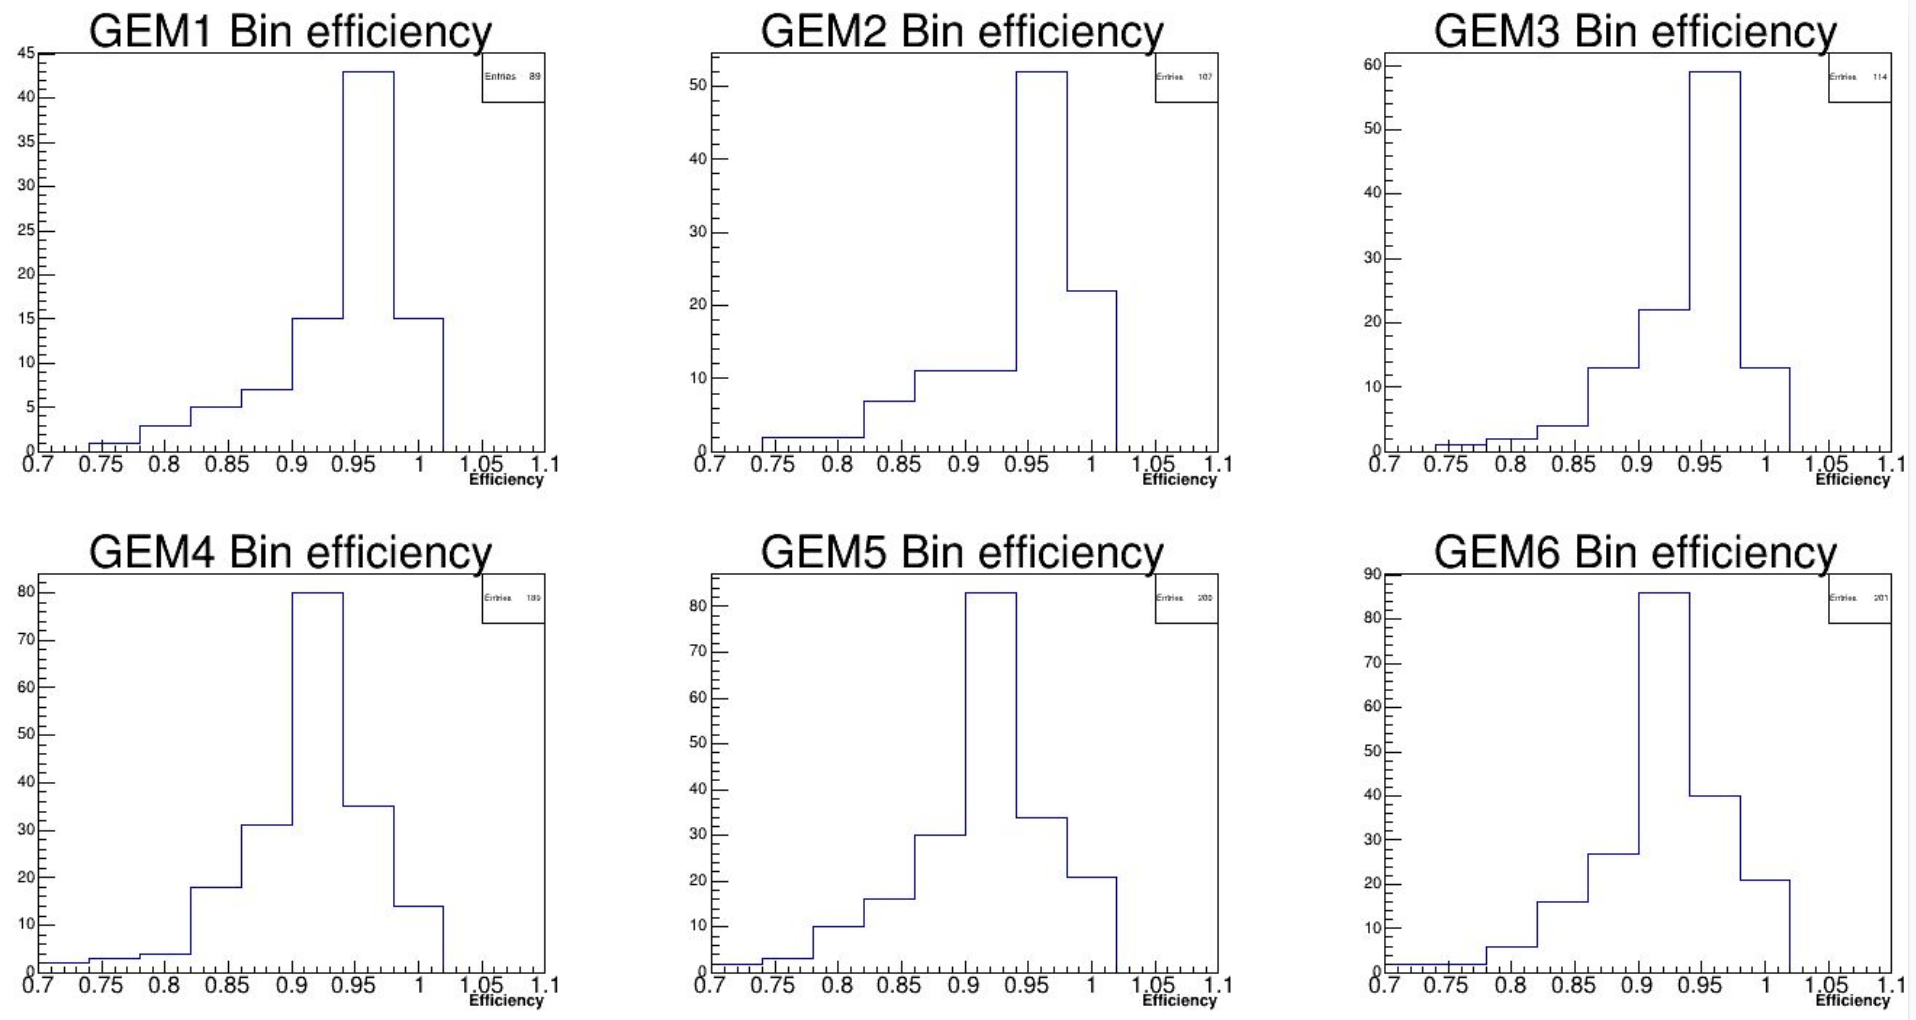
\includegraphics[width=\textwidth]{images/chap5/rhrs_gem_bin_efficiency.png}
    \caption{GEM Efficiency distribution}
    \label{fig:rhrs_gem_bin_efficiency}
\end{figure}

\subsubsection{GEM detector efficiency over time}

GEM detector efficiency increase with time [TO BE ADDED]. 

%
% NL: edits on 07/14
%
\subsubsection{GEM detector High Rate Performance and compare with VDC}
In a gas ionization detector, while the ionized electrons drift the the anode strips or wires, the created positive ions drift in the opposite direction along the electric field. Given their much heavier mass, the drift velocity of the positive ions is significantly less than that of the electrons. As such, the time it takes the positive ions to drift back and get removed from the detector volume act as the limiting factor on the detector rate. 

The GEM foil is a two-layer copper-coated structure, with avalanches occurring only inside the holes of the GEM foil. Most Ionized ions are absorbed by the copper layers, reducing the travel distance  for the ions to at most 70 µm. This is a significant reduction compared to the drift chamber, which is limited in its maximum event rate due to the much longer drift time of the ions over many mm. The maximum working rate for the drift chamber is limited to approximately few kHz.cm$^2$, whereas the GEM detector's event rate can reach MHz per square centimeter. 

The GEM detector can achieve a higher event rate than the drift chamber due to its smaller drift time for ions. In the event rate measurement, both GEM and VDC detectors are used for tracking. However, for safety concerns, when the event rate exceeds 500 kHz, only the GEM detector is employed.

Since the VDC detectors are  not used when the event rate is greater than 500 kHz, a consistent efficiency is obtained by reconstructing the track with six layers of GEM detectors for the efficiency measurement. The VDC efficiency is measured by projecting the GEM track back to the VDC plane and searching for fired events on the VDC detector. Similarly, the GEM efficiency calculation is performed by projecting the track to each GEM detector and searching for fired events in each GEM detector plane.

Figure \ref{fig:apv_25_pedestal_plot} shows the comparison of the GEM detector and VDC detector  efficiency  at different event rates. The blue points represent the efficiency of the VDC detectors, while the red points represent the efficiency of the GEM detectors. Within the test range from 20 kHz(?) to 1.5 MHz(?), the efficiency of the GEM detector remains consistent. On the other hand, the efficiency of the VDC detector decreases as the event rate increases, dropping to around $60\%(?)$ when the event rate reaches 500 kHz. 
%
% NL note to Siyu: Since we normally quote the rates per cm^2; it would be nice to estimate
% what this integrated rate of 500 kHz corresponds to at the elastic peak location. to do 
% this take a small area at the peak and consider the rate within that area 
%

[add all the GEM detectors]



\begin{figure}[!htbp]
    \centering
    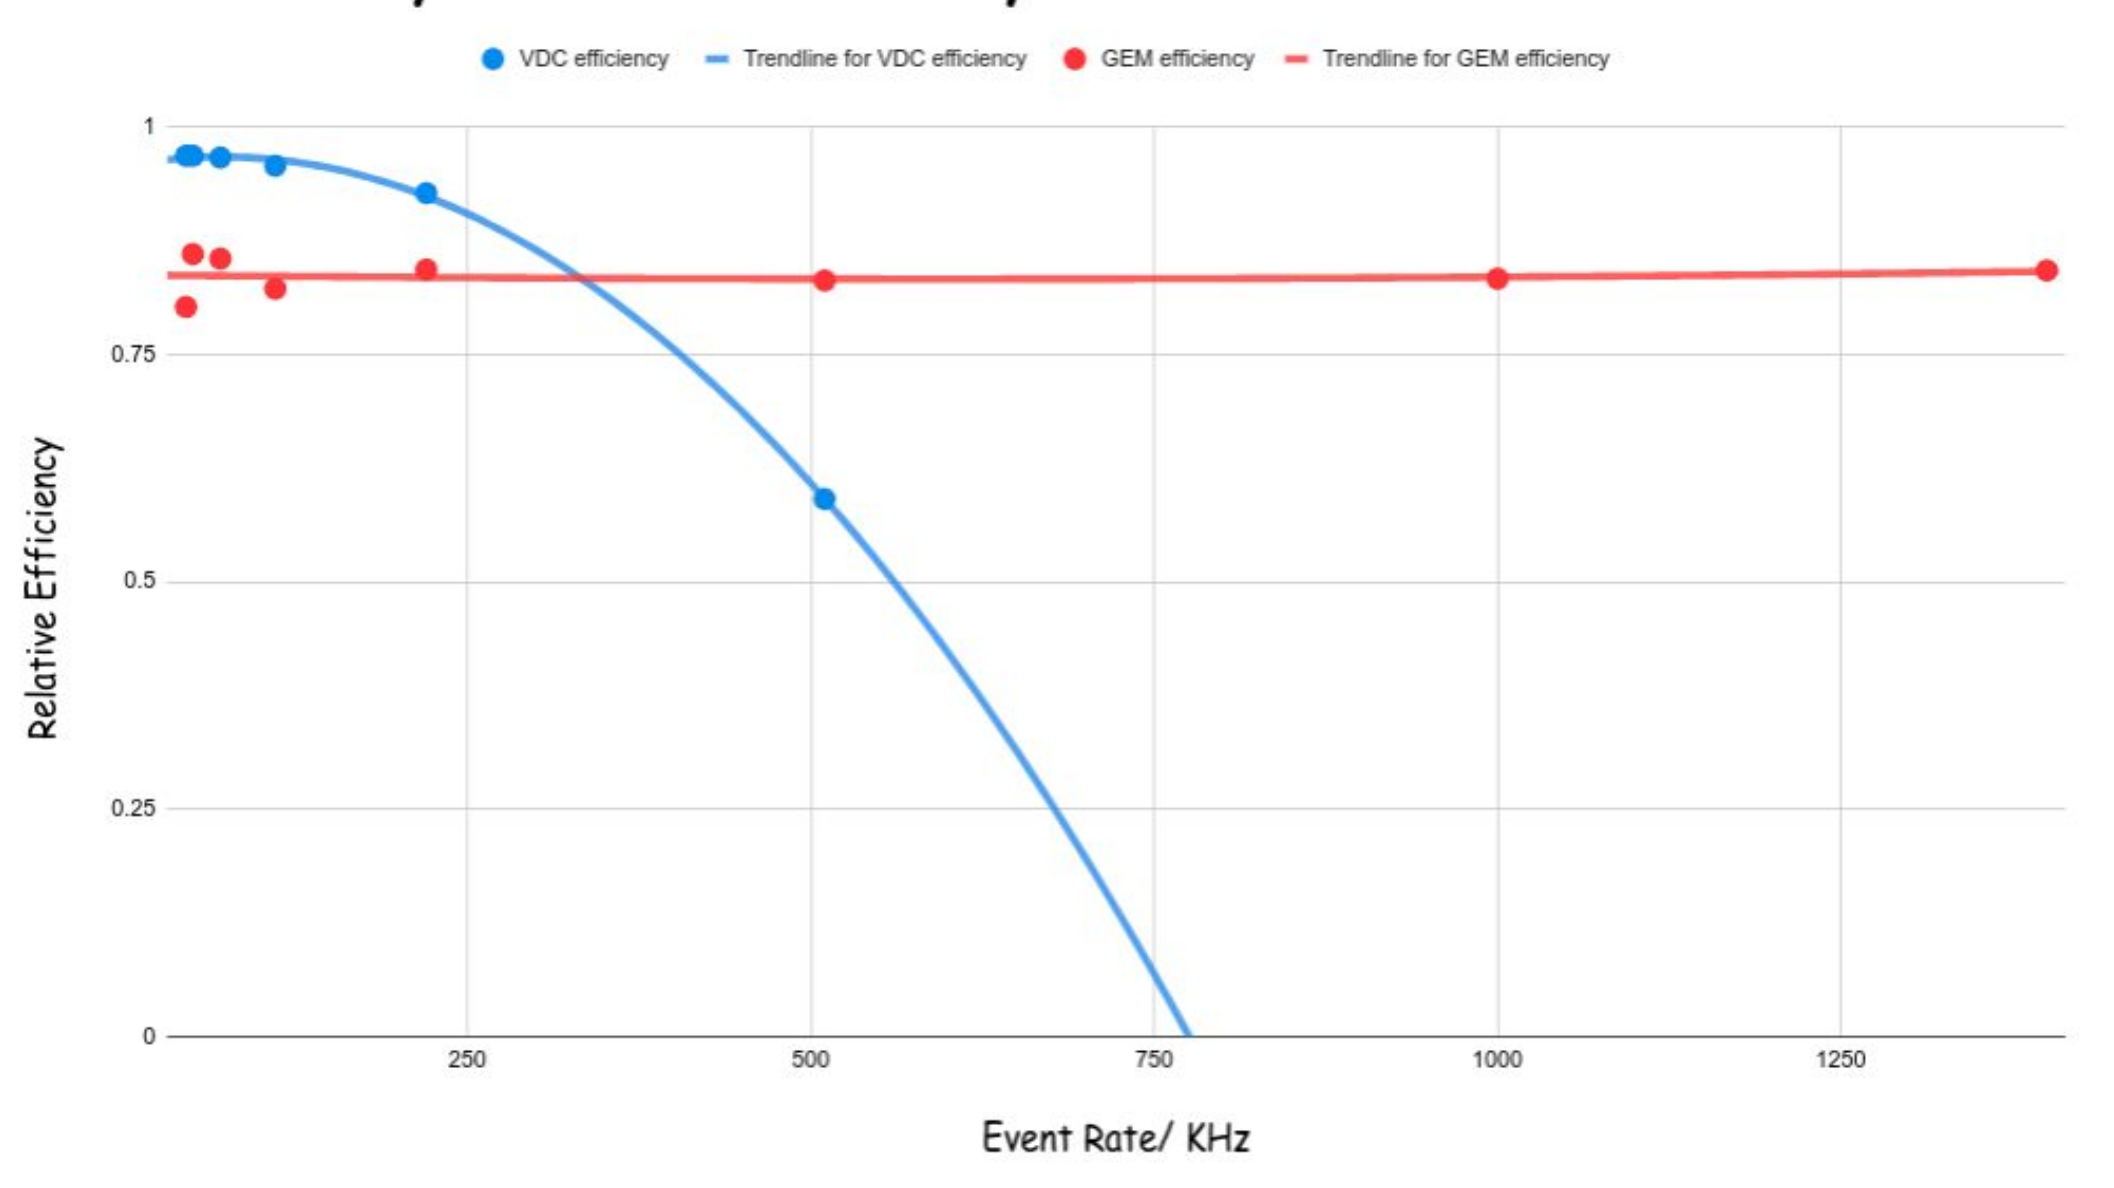
\includegraphics[width=\textwidth]{images/chap5/gem efficiency over time.png}
    \caption{GEM and VDC efficiency Over Time}
    \label{fig:gem_efficiency_over_time}
\end{figure}